\documentclass[a4paper]{report}

\usepackage{graphicx}
\usepackage{wrapfig}
\usepackage{url}
\usepackage{listings}
\usepackage{color}
\usepackage{lipsum}
\usepackage{hyperref}
\usepackage{float}

\definecolor{darkgreen}{rgb}{0,0.6,0}
\definecolor{darkorange}{rgb}{1,0.4,0}

\lstdefinestyle{codestyle}{
    backgroundcolor=\color{white},
    commentstyle=\color{darkgreen},
    keywordstyle=\color{blue},
    numberstyle=\color{black},
    stringstyle=\color{darkorange},
    basicstyle=\ttfamily\footnotesize,
    breakatwhitespace=false,
    breaklines=true,
    captionpos=b,
    keepspaces=true,
    numbers=left,
    showspaces=false,
    showstringspaces=false,
    showtabs=false,
    breaklines=true,
}

\lstset{style=codestyle}

\hypersetup{
    hidelinks
}

\author{Emanuele Franchi}
\title{Exploring The Vulkan Graphics API}

\begin{document}

\emergencystretch 5em

\maketitle

\chapter*{Abstract}
Thesis about Vulkan

\chapter*{Dedication}
Bla Bla Bla

\chapter*{Acknowledgments}
I want to thank...

\tableofcontents
\listoffigures
\lstlistoflistings

\chapter{Vulkan}

\section{OpenGLBook Notes}

On the most fundamental level, OpenGL (graphics APIs in general) is a software
interface that allows a programmer to communicate with graphics hardware.

The first Personal Computers started to appear in the mid to late 1970s,
but were regarded as enthusiast machines for hobbyists.
This changed somewhat with the release of the Apple II by Apple Computer in
1977, and the PET by Commodore International. These machines popularized the
concept of computers for the home, but did not have too much to offer in terms
of computer graphics.

This somewhat changed in the 1980s when technologies such as GUI were introduced
to the personal computing market. The first dedicated graphics add-on cards also
started to appear during this era, notably the CGA (Color Graphics Adapter)
by IBM was the first color graphics card for the IBM PC platform, which
would pave the way for future developments by standardizing a method of drawing
computer graphics but didn't offer much in terms of graphics capabilities.

During the 1970s and 1980s, most video games ran on specialized systems,
movies made use of computer animation only sparsely, and real-time 3D
graphics were for visualization purposes only since there was no consumer
hardware that was fast enough.
These years were known for their many firsts on consumer hardware, but
it wasn't until the late 1980s to the early 1990s when computer games took
a strong hold on the PC platform and a real push for better looking and better
performing real-time graphics began.

Silicon Graphics (commonly referred to as SGI) was a company founded in
1981 that specialized in 3D computer graphics and developed software and hardware
specifically for this purpose. One software library that SGI developed was
IRIS GL (Integrated Raster Imaging System Graphical Library) used for generating
2D and 3D graphics on SGI's high performance workstations.

In the early 1990s, SGI was the market leader in 3D graphics workstations
because of their high performance hardware and easy to use software.
IRIS GL was the de facto industry standard 3D graphics library, overshadowing
all other developments and attempts to standardize a 3D graphics interface.
But despite its popularity, IRIS GL had one major problem: it was a proprietary
system fused to SGI's own platforms, and competitors were closing in on SGI's
advantage with their own APIs.

In a bold move, SGI cleaned up IRIS GL, removed all functionality that
did not relate to computer graphics and released it to the public in 1992 as
OpenGL (Open Graphics Library), a cross-platform standardized API for real-time
computer graphics.

Software vendors would have to provide their own implementations of the
OpenGL standard on their platforms, and hardware vendors programs that
allowed OpenGL to talk to the underlying graphics hardware called "device drivers".

The name "OpenGL" was not just chosen because it sounded like a fine buzzword,
it also contains some actual meaning. Since OpenGL is an evolving specification,
someone has to decide what goes in it. So in 1992, the ARB (OpenGL Architecture
Review Board) was founded, which comprised of several high profile software and
hardware vendors who collectively decided the future of the OpenGL standard through
a voting system. Besides determining what new features went into the OpenGL
specification, it also decided which extensions would be promoted to become
core features of the next OpenGL release.

OpenGL quickly became the industry leading real-time graphics API,
as it was basically the only one available on multiple platforms.

In the late 1990s, OpenGL established itself as an industry standard for
3D computer graphics, not just for CAD programs, although it was the only
contender in that market. PC video games such as Quake 2, Unreal, and Half-Life
took full advantage of OpenGL to show off their full potential and were widely
popular. Around this time, the first consumer-grade dedicated 3D graphics
hardware started to appear, changing the video game industry forever.

During the early 2000s, GPU performance grew exponentially as more software
features were moved to the GPU. The CPU became obsolete for rendering real-time
3D graphics since it could not keep up with GPU developments. In fact, the current
method of rendering 3D graphics saw the CPU as such major bottleneck that new
methods had to be invented to circumvent its use.

In rendering real-time computer graphics, the software pipeline exists to
describe what we'd like to see on the screen.
For example, if we'd like to display a green square on the screen,
computer software would describe with which dimensions, color, and at which
position of the screen to draw the square.

The software pipeline also provides access to functionality that draws
the geometry onto the screen. It is worth noting that the software pipeline
does not actually do any drawing or transformations, since on modern systems
this functionality is entirely implemented by the hardware.

The software pipeline consists of several different layers, each with their
own very specific purposes.

The first is the Application layer, which is your program, the program that
invokes drawing commands. The application serves as a controller of the overall
process and oversees all of the user-level operations such as creating windows,
threads, memory allocation, complex user data-types, and making calls to external
libraries such as OpenGL or Direct3D through their respective interfaces.

The next layer is the Abstraction layer, which contains the OpenGL or Direct3D
API implementations.
The Abstraction layer serves as a dispatch to the next layer by implementing
hardware-level functionality in a usable and standardized format.

The abstraction layer passes its commands to the Device Driver, a software
communication layer to the hardware. This layer is entirely invisible to the
developer, since it cannot be interacted with through your program.
The device driver interprets the commands passed to it by the Abstraction
layer and relays them to the underlying device in a format that the hardware
can understand and easily process.

\section{Learn WebGL}

In the early days, if you wanted to create computer graphics you had to
write programs that directly talked to the graphics hardware. As new hardware
designs were created, the software had to be completely re-written to work with
the new hardware.

The premiere computer graphics company in the late 1980's and throughout
the 1990's was Silicon Graphics, Inc. They were a hardware company, but
they shipped their computers with a proprietary computer graphics application
programmer interface (API) known as IRIS Graphics Language (IRIS GL).

\section{Graphics Book}

In the first desktop computers, the contents of the screen were managed
directly by the CPU. For example, to draw a line segment on the screen, the CPU
would run a loop to set the color of each pixel that lies along the line.
Needless to say, graphics could take up a lot of the CPU's time. And graphics
performance was very slow, compared to what we expect today. So what has changed?
Computers are much faster in general, of course, but the big change is that in
modern computers, graphics processing is done by a specialized component called
a GPU, or Graphics Processing Unit. A GPU includes processors for doing graphics
computations; in fact, it can include a large number of such processors that work
in parallel to greatly speed up graphical operations. It also includes its own
dedicated memory for storing things like images and lists of coordinates.
GPU processors have very fast access to data that is stored in GPU memory—much
faster than their access to data stored in the computer's main memory.

To draw a line or perform some other graphical operation, the CPU simply
has to send commands, along with any necessary data, to the GPU, which
is responsible for actually carrying out those commands. The CPU offloads most
of the graphical work to the GPU, which is optimized to carry out that work very
quickly. The set of commands that the GPU understands make up the API of the GPU.
OpenGL is an example of a graphics API, and most GPUs support OpenGL in the sense
that they can understand OpenGL commands, or at least that OpenGL commands can
efficiently be translated into commands that the GPU can understand.

\section{History of Computer Graphics}

Computer Graphics (CG) was first developed as a visualization tool.
Computer graphics were basically introduced for scientists and engineers
in government and corporate research centers.

\section{In a Nutshell: History of OpenGL}

Application programming interfaces define how applications interact with
the hardware components of a computer. They define a set of subroutines,
protocols and tools for building application software. The main goal of an
API is to abstract the underlying implementation of software and hardware and
provide the developer the tools to interact with them. Graphics APIs are
implemented by driver software that is written by graphics hardware vendors
specifically for each hardware. They are the medium with which developers can
control the dedicated graphics hardware by issuing various
implementation-agnostic, higher-level commands to the software driver
who in turn translates them to lower level commands for each specific
hardware. The next sections of this post will talk about OpenGL,
the group that created it, its history and its design philosophies.

OpenGL has been developed for over 26 years and that is a significant
amount of time in the development of cutting-edge technology.
Back in 1992 the best Intel CPU was the 80486 and math coprocessors
were an optional component. Apple computers were using Motorola
68K-derived processors and PowerPC processors were not available until
the second half of 1992. Home personal computers did not have any kind of
high-performance hardware graphics acceleration. The only way to access this
rare luxury and be able to use OpenGL was through an expensive workstation.
The state of the art in graphics was using software rendering. The best that
could be achieved without hardware acceleration was a small amount of simple
colored, filled polygons.

As time passed, the prices of graphics hardware declined, and their
performance increased. Furthermore, new features were added to the now
low-cost graphics processors which in turn were added to the OpenGL specifications
as well. Those extra features were initially added to OpenGL as extensions
which were proposed by members of the OpenGL ARB. Some of these extensions
interacted well with each other and with already existing feature of OpenGL
and some did not. Moreover, as newer ways of taking advantage of the GPU were
invented they were added in OpenGL as well, resulting in having multiple ways
available to do the same thing.

\section{Red Book}

In the very old days, drawing graphics was slow. The only way to draw graphics
quickly was to get a super computer. The early special effects companies
went bankrupt because they tried to buy Crays and things like that.
In the late 1970s and early 1980s, workstations started to be produced
commercially.

In the late 1970s, a professor at Stanford (Jim Clark) had the idea to
try to build specialized hardware to do graphics (relatively) fast and fit
it into a workstation. The plan was based on the existence of special chips
for performing certain mathematical operations (like a chip for doing 4x4
matrix multiplies). He and his students started a company to bring the
machines to market. The company was called Silicon Graphics (SGI).

SGI was really successful in the late 1980s and early-mid 1990s.
They dominated the graphics hardware market. Most interesting graphics software
ran on their hardware. It was the machine you wanted to have if you were doing
graphics.

In the mid- to late- 1990s, other companies realized that GL was a good
way to program graphics, and wanted to let programmers work that way.
So, a standards group was formed and they created OpenGL. OpenGL was designed
so that it didn't require SGIs hardware and operating system. But, it worked
like GL, which was designed with SGI's hardware in mind. Mostly this was a
good thing (since the hardware was based on good ways to think about graphics).
But some things were weird, because the hardware did things in a
weird way (like lighting). And some features were really historical: they were
designed to support what early 1990s SGI hardware did, and the best way to use that.

For a while, this was great. We had a convenient way to program graphics
that worked across different platforms.
But then, graphics hardware evolved. Very quickly. OpenGL had to be extended
to provide people with access to these new features.

But worse, while the old ways of programming graphics (i.e. what the SGI
hardware did in 1990) was convenient for many things, and was the most efficient
way to do stuff for circa 1990 computers, it was not at all how modern hardware
worked. In fact, it was quite inefficient since it was based on assumptions
about what is fast and slow that are very different than the are now.

So, in the late 2000s, early 2010s, the folks in charge of OpenGL decided to
remove all of the old circa 1980s/1990s stuff designed for SGI hardware.
They call this part of OpenGL "legacy" OpenGL.

\section{What is Vulkan?}

\begin{wrapfigure}{l}{0.4\textwidth}
    \begin{center}
        
\includegraphics[scale=0.10]{images/ChVulkan/VulkanLogo.png}
    \end{center}
    \caption{Vulkan logo}
    \label{fig:VulkanLogo}
\end{wrapfigure}

Vulkan is a modern graphics API. It is maintained by the Khronos Group.
Vulkan is meant to abstract how modern GPUs work.
Using Vulkan, the programmer can write more performant code.
The better performance comes at the cost of having a more verbose and low level API compared to
other existing APIs such as OpenGL or Direct3D 11 and prior.
Vulkan is not the only modern graphics API, other such APIs are Direct3D 12 and Metal.
Nonetheless, Vulkan has the advantage of being fully cross platform.

\section{What problems does Vulkan solve?}

\begin{wrapfigure}{l}{0.4\textwidth}
    \begin{center}
        
\includegraphics[scale=0.10]{images/ChVulkan/OpenGLLogo.png}
    \end{center}
    \caption{OpenGL logo}
    \label{fig:OpenGLLogo}
\end{wrapfigure}

Common graphics APIs like OpenGL or Direct3D were developed during the 1990s.
At that time, graphics card hardware was very limited not only in terms of computational
power but also from a functionality standpoint. As time progressed, graphics card architectures
continued to evolve, offering new functionalities.
All these new functionalities had to be integrated with the old existing APIs.
The more new functionalities were integrated, the more the GPU's driver complexity grew.
Such complicated GPU drivers are inefficient and are also the cause of many
inconsistencies between implementations of the same graphics API but on different GPUs.

\section{How does Vulkan solve these problems?}

Vulkan doesn't suffer from the problems we saw above because it has been designed from scratch
and with modern GPU's architecture in mind.
It reduces the driver overhead by being more verbose and low level.
It is also designed to be multithreaded, allowing the programmer to submit GPU commands from
different threads.
This is very beneficial to performance, since modern CPUs usually have more than one core.

\chapter{Initializing Vulkan}

TODO: chapter introduction ...

\section{Create Vulkan Instance}

To access any of the functionalities offered by Vulkan we first have to create a Vulkan
instance.
To do this we call vkCreateInstance.

\begin{minipage}{\linewidth}{\noindent}
    \lstinputlisting[
        language=C++,
        caption={Create Vulkan instance},
        label={lst::CreateInstance}
        ]{src/ChInitializingVulkan/CreateInstance.cpp}
\end{minipage}

\subsection{VkInstanceCreateInfo}

To call vkCreateInstance we need to pass a pointer to a VkInstanceCreateInfo struct.
This struct collects all the information needed to configure our Vulkan instance.

\begin{minipage}{\linewidth}{\noindent}
\lstinputlisting[
    language=C++,
    caption={VkInstanceCreateInfo initialization},
    label={lst::VkInstanceCreateInfo}
    ]{src/ChInitializingVulkan/VkInstanceCreateInfo.cpp}
\end{minipage}

\subsection{VkApplicationInfo}

We can see that the VkInstanceCreateInfo struct is not the only thing we need.
We have to specify a pointer to a VkApplicationInfo struct. Such struct describes
our Vulkan application.

\begin{minipage}{\linewidth}{\noindent}
    \lstinputlisting[
        language=C++,
        caption={VkApplicationInfo initialization},
        label={lst::VkApplicationInfo}
        ]{src/ChInitializingVulkan/VkApplicationInfo.cpp}
\end{minipage}

\subsection{Layers}

While we initialize our VkInstanceCreateInfo struct, we can specify the layers
that we want to enable.
The specified layers will be loaded after the Vulkan instance creation.

Layers are optional components that hook into Vulkan.
Layers can intercept, evaluate and modify existing Vulkan functions.
Layers are implemented as libraries and are loaded during instance creation.

If we want to enable error checking, we need to load a layer that
provides such functionality.
This kind of layer is know as validation layer.
There are different validation layers.
Here follows an example. Since validation layers cause overhead, we can
disable them when we build the application in release mode.

\begin{minipage}{\linewidth}{\noindent}
    \lstinputlisting[
        language=C++,
        caption={Enabling the Khronos validation layer},
        label={lst::ValidationLayer}
        ]{src/ChInitializingVulkan/ValidationLayer.cpp}
\end{minipage}

\subsubsection{Checking whether our layers are supported}

Before creating our Vulkan instance, we should check if the layers we require are
actually supported.
To do this we use vkEnumerateInstanceLayerProperties.
This function returns all the layers supported by our Vulkan installation.
If all the layers we require are present, then we can proceed to create our
Vulkan instance.

\subsection{Extensions}

While we initialize our VkInstanceCreateInfo struct, we can specify the instance
extensions that we want to enable.
The specified instance extensions will be loaded after the Vulkan instance creation.

Extensions are  additional features that Vulkan implementations may provide.
Extensions add new functions and structs to the API.
Extensions may also change some of the behavior of existing functions.
We can either enable extensions at an instance level or at a device level.

We can use an extension to provide a callback to handle the debug messages
generated by the validation layers.

\begin{minipage}{\linewidth}{\noindent}
    \lstinputlisting[
        language=C++,
        caption={Enabling an extention to handle validation layer debug messages},
        label={lst::DebugExtension}
        ]{src/ChInitializingVulkan/DebugExtension.cpp}
\end{minipage}

We specify one callback that handles messages generated by
instance creation and destruction.
We also specify another callback that handles all other API debug messages.

\begin{minipage}{\linewidth}{\noindent}
    \lstinputlisting[
        language=C++,
        caption={Setting up debug extension callbacks},
        label={lst::DebugExtensionCallbacks}
        ]{src/ChInitializingVulkan/DebugExtensionCallbacks.cpp}
\end{minipage}

The function that creates the VkDebugUtilsMessengerEXT object comes from the
extension we have enabled.
Because of this, we have to load it manually into our address space using
vkGetInstanceProcAddr.
An elegant way to solve this issue us to create a proxy function that handles
this matter for us.

\begin{minipage}{\linewidth}{\noindent}
    \lstinputlisting[
        language=C++,
        caption={Extension function proxy},
        label={lst::ExtensionFunctionProxy}
        ]{src/ChInitializingVulkan/ExtensionFunctionProxy.cpp}
\end{minipage}

\subsubsection{Checking whether our extensions are supported}

Before creating our Vulkan instance, we should check if the instance extensions
we require are actually supported.
To do this we use vkEnumerateInstanceExtensionProperties.
This function returns all the instance extensions that are supported by our
Vulkan installation.
If all the instance extensions we require are present, then we can proceed to
create our Vulkan instance.

\subsection{Vulkan Instance Cleanup}

When our application is shutting down, we destroy the debug messenger
and destroy our vulkan instance. DestroyDebugUtilsMessengerEXT is an extension
function proxy.

\begin{minipage}{\linewidth}{\noindent}
    \lstinputlisting[
        language=C++,
        caption={Vulkan Instance Cleanup},
        label={lst::InstanceCleanup}
        ]{src/ChInitializingVulkan/InstanceCleanup.cpp}
\end{minipage}

\section{Open A Window}

After creating our Vulkan instance we open a window.
To do this we have two options.
We can use a cross platform library that will do all the heavy lifting
for us, so that we don't have to worry about directly interacting with the OS,
freeing us from the burden of knowing how its windowing API works.
We can also decide to not use a library and opening the window ourselves.
We will do the latter, since it's interesting to know how things work under the surface.

Since I'm on Windows, I'll be dealing with the Win32 API.
We won't go in depth about the specifics of this API since it's beyond our scope.

\subsection{Create Window Handle}

To create a handle to a window we use CreateWindowEx.
We use windowStyle and windowExtendedStyle variables to configure how we want our window.

\begin{minipage}{\linewidth}{\noindent}
    \lstinputlisting[
        language=C++,
        caption={Creating a window handle using Win32 API},
        label={lst::CreateWindowEx}
        ]{src/ChInitializingVulkan/CreateWindowEx.cpp}
\end{minipage}

\subsection{Computing Window Dimensions}

Before creating our window, we need to compute its width and height.
This is due to the fact that a window comprises of a client area and a non client area.
We usually want our client area to be of a certain size, but CreateWindowEx takes
the whole window width and the whole window height as arguments.

\begin{figure}[ht]
    \centering
    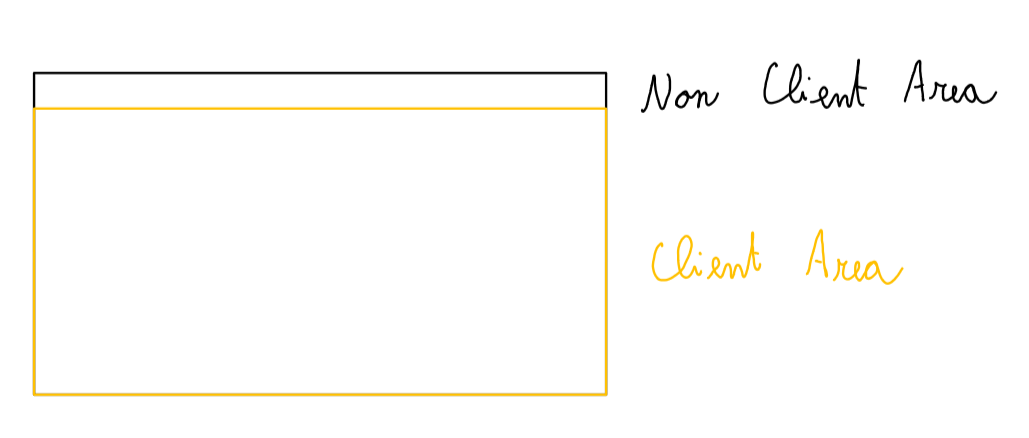
\includegraphics[scale=0.30]{images/ChInitializingVulkan/Win32Window.png}
    \caption{Anatomy of a Win32 Window}
    \label{fig::Win32Window}
\end{figure}

\begin{minipage}{\linewidth}{\noindent}
    \lstinputlisting[
        language=C++,
        caption={Compute window width and height},
        label={lst::AdjustWindowRectEx}
        ]{src/ChInitializingVulkan/AdjustWindowRectEx.cpp}
\end{minipage}

\subsection{Register Window Class}

Before creating our window, we need to register its window class.
To do this we use RegisterClassEx.
This function takes a pointer to a WNDCLASSEX struct.
This struct is used to configure our window class;

\begin{minipage}{\linewidth}{\noindent}
    \lstinputlisting[
        language=C++,
        caption={Register Window Class},
        label={lst::RegisterClassEx}
        ]{src/ChInitializingVulkan/RegisterClassEx.cpp}
\end{minipage}

\subsection{Window Procedure}

While filling in our WNDCLASSEX struct, we also passed a WindowProcedure.
This is a callback function that we have to define.
We use this function to handle the events that our window will receive during
the lifespan of our application.

The Win32 API also provides a default window procedure.
Our custom window procedure will call this default procedure when we don't want
to handle particular events ourselves.

\begin{minipage}{\linewidth}{\noindent}
    \lstinputlisting[
        language=C++,
        caption={Window Procedure},
        label={lst::WindowProcedure}
        ]{src/ChInitializingVulkan/WindowProcedure.cpp}
\end{minipage}

\subsection{Window Cleanup}

When our application is shutting down, we destroy our window and unregister
its class.

\begin{minipage}{\linewidth}{\noindent}
    \lstinputlisting[
        language=C++,
        caption={Window Cleanup},
        label={lst::WindowCleanup}
        ]{src/ChInitializingVulkan/WindowCleanup.cpp}
\end{minipage}

\section{Create A Presentation Surface}

We must link our newly created window to our Vulkan instance.
To do this we create a presentation (or window) surface.
This operation is platform specific.
Since we are using Windows, to create our presentation surface we need
to use vkCreateWin32SurfaceKHR.

\begin{minipage}{\linewidth}{\noindent}
    \lstinputlisting[
        language=C++,
        caption={Create Presentation Surface},
        label={lst::CreatePresentationSurface}
        ]{src/ChInitializingVulkan/CreatePresentationSurface.cpp}
\end{minipage}

\subsection{VkWin32SurfaceCreateInfoKHR}

When we call vkCreateWin32SurfaceKHR, we need to pass a pointer to a
VkWin32SurfaceCreateInfoKHR struct.
Such struct lets us configure our presentation surface creation.

\begin{minipage}{\linewidth}{\noindent}
    \lstinputlisting[
        language=C++,
        caption={Filling in a VkWin32SurfaceCreateInfoKHR struct},
        label={lst::VkWin32SurfaceCreateInfoKHR}
        ]{src/ChInitializingVulkan/VkWin32SurfaceCreateInfoKHR.cpp}
\end{minipage}

\subsection{Required Instance Extensions}

Vulkan, being cross platform, cannot interact directly with the OS windowing system.
To do this we use extensions.

The first extension that we enable is the instance level KHR surface extension.
This extension exposes a VkSurfaceKHR object that represents a surface to present
rendered images to.
This surface will be backed by the window we have created.

The second extension we enable is platform specific and is needed
to create our VkSurfaceKHR object.
In our case, since we are using Windows, we enable the instance level KHR win32
surface extension.

\begin{minipage}{\linewidth}{\noindent}
    \lstinputlisting[
        language=C++,
        caption={Presentation Surface Extensions},
        label={lst::PresentationSurfaceExtensions}
        ]{src/ChInitializingVulkan/PresentationSurfaceExtensions.cpp}
\end{minipage}

Notice the define preprocessor directive right before including our Vulkan header.
We do this to access our native platform functions.

\subsection{Presentation Surface Cleanup}

When our application is shutting down, we destroy our presentation surface.

\begin{minipage}{\linewidth}{\noindent}
    \lstinputlisting[
        language=C++,
        caption={Presentation Surface Cleanup},
        label={lst::PresentationSurfaceCleanup}
        ]{src/ChInitializingVulkan/PresentationSurfaceCleanup.cpp}
\end{minipage}

\section{Pick A Physical Device}

Now that we have a Vulkan instance and a presentation surface, we select
a physical device (a GPU) that supports the features we need.
The selected GPU will be the one that will be used by our application.

\subsection{Listing Available Physical Devices}

We first get a list of all the physical devices that are available on the
system.
To do this we use vkEnumeratePhysicalDevices.
These physical devices can either be integrated or dedicated GPUs.

\subsection{Finding A Suitable Physical Device}

Now that we have a list of all the physical devices, we can select one of them.
We could, for example, automatically pick the first one without doing any kind
checking.
This approach is doable if we don't have any particular requirement for our
physical devices.

Usually we have a set of specific physical device features that are mandatory
for our application to run.
Hence, in our list, some physical devices will be suitable for our application, while
others won't.

The approach we take here is to iterate through the list of all physical devices and
picking the first one that is suitable for our application.
One question still remains: how can we tell if a physical device is suitable or not?

\subsubsection{Spport Grpahics Operations}

To check if our physical device supports graphics operations we list all
the queue families of our physical device.
To do this we use vkGetPhysicalDeviceQueueFamilyProperties.
Then we check if at least one queue family supports graphics operations.

\begin{minipage}{\linewidth}{\noindent}
    \lstinputlisting[
        language=C++,
        caption={Check for graphics operations support},
        label={lst::SupportGraphicsOperations}
        ]{src/ChInitializingVulkan/SupportGraphicsOperations.cpp}
\end{minipage}

\subsubsection{Spport Present Operations}

To check if our physical device supports present operations we list all
the queue families of our physical device.
To do this we use vkGetPhysicalDeviceQueueFamilyProperties.
Then we check if at least one queue family supports present operations.

\begin{minipage}{\linewidth}{\noindent}
    \lstinputlisting[
        language=C++,
        caption={Check for present operations support},
        label={lst::SupportPresentOperations}
        ]{src/ChInitializingVulkan/SupportPresentOperations.cpp}
\end{minipage}

\subsubsection{Support Presentation To A Surface}

Not only our physical device must support present operations.
It must also be able to present images to the screen.
Image presentation is tied to the window and consequently to the surface
associated with it.
For this reason, image presentation to the screen is not part of Vulkan.
We have to enable the KHR swapchain device extension to support such operation.
We need this extension because image presentation to a surface is achieved using
a swapchain.

\begin{minipage}{\linewidth}{\noindent}
    \lstinputlisting[
        language=C++,
        caption={Device extension for image presentation to the screen},
        label={lst::DeviceExtensions}
        ]{src/ChInitializingVulkan/DeviceExtensions.cpp}
\end{minipage}

As we have seen earlier, before enabling an extension, we should check for its
support.
To check whether our physical device supports one or more device extensions we use
vkEnumerateDeviceExtensionProperties.
This function returns a list of all the extensions supported by our physical device.
Then, we simply check whether all the extensions we require are present in the list.

\subsubsection{Support A Present Mode}

Checking if a swapchain is supported is not sufficient.
Even if it's supported, it may not be compatible with our presentation surface.
We need to check whether our physical device supports at least one present mode
for our presentation surface.
We can do this using vkGetPhysicalDeviceSurfacePresentModesKHR.
This functions returns a list of present modes supported by our physical device
that are compatible with our presentation surface.
If there is at least one present mode in the list, then we are good to go.

\section{Create A Logical Device}

\section{Create A Swapchain}

\chapter{Clear The Window}

\chapter{Rendering Our First Triangle}

In this chapter we see how to render a triangle on the screen.
This is the classic computer graphics hello world program.
If we are able to draw a single triangle, then we can draw almost any shape.
We can do this by considering the shape we want to draw as if it were
made up of one or more triangles and then drawing them.

In order to render a triangle using Vulkan, we have to set up a pipeline state
object.
This object describes the entire state of our pipeline.
Thus, it also describes how we want to draw something.
In our application main loop, during our command buffer recording, we
simply need to use a pipeline state object and issue a draw call that activates
our pipeline.

\section{Create A Pipeline State Object}

To create a pipeline state object we use \texttt{vkCreateGraphicsPipelines}.

\begin{minipage}{\linewidth}{\noindent}
    \lstinputlisting[
        language=C++,
        caption={Create a pipeline state object},
        label={lst::CreatePipelineStateObject}
        ]{src/ChTriangle/CreatePipelineStateObject.cpp}
\end{minipage}

\subsection{VkGraphicsPipelineCreateInfo}

We use a \texttt{VkGraphicsPipelineCreateInfo} struct to configure the pipeline state
object we are about to create.

\texttt{layout} is the description of binding locations used by both the pipeline
and descriptor sets used with the pipeline.
It doesn't matter in our case.
We will see its use when we talk about uniforms.

\texttt{renderPass} is a handle to a render pass object describing the environment
in which the pipeline will be used.

\texttt{subpass} is the index of the subpass in the render pass where
this pipeline will be used.

We will explain the meaning of the remaining relevant struct fields
in the next sections.

\begin{minipage}{\linewidth}{\noindent}
    \lstinputlisting[
        language=C++,
        caption={Configure pipeline state object},
        label={lst::VkGraphicsPipelineCreateInfo}
        ]{src/ChTriangle/VkGraphicsPipelineCreateInfo.cpp}
\end{minipage}

\subsection{Shader Stages}

We have to specify a collection of all shader stages and shader programs that
will be used during rendering.

\begin{minipage}{\linewidth}{\noindent}
    \lstinputlisting[
        language=C++,
        caption={Shader stages},
        label={lst::ShaderStages}
        ]{src/ChTriangle/ShaderStages.cpp}
\end{minipage}

\subsubsection{VkPipelineShaderStageCreateInfo}

In our case we need two instances of a \texttt{VkPipelineShaderStageCreateInfo}
struct that describe our vertex and our fragment shader stages.

\texttt{stage} is a \texttt{VkShaderStageFlagBits} value specifying the
pipeline stage.
\texttt{module} is a shader module object containing the shader for this stage.
\texttt{pName} is a string specifying the entry point name of the shader for this
stage.

\begin{minipage}{\linewidth}{\noindent}
    \lstinputlisting[
        language=C++,
        caption={Describe a shader stage},
        label={lst::VkPipelineShaderStageCreateInfo}
        ]{src/ChTriangle/VkPipelineShaderStageCreateInfo.cpp}
\end{minipage}

In order to create our vertex shader stage we need to pass the shader module
that contains our vertex shader code and use the
\texttt{VK\_SHADER\_STAGE\_VERTEX\_BIT} stage flag bit.

In order to create our fragment shader stage we need to pass the shader module
that contains our fragment shader code and use the
\texttt{VK\_SHADER\_STAGE\_FRAGMENT\_BIT} stage flag bit.

\subsubsection{VkShaderModule}

To create a shader module we need to load our shader code written
in SPIR-V binary format.
Then, we simply use \texttt{vkCreateShaderModule}.
After creating our shader module, we can discard our loaded shader code.

\begin{minipage}{\linewidth}{\noindent}
    \lstinputlisting[
        language=C++,
        caption={Create a shader module},
        label={lst::VkShaderModule}
        ]{src/ChTriangle/VkShaderModule.cpp}
\end{minipage}

In our case, we create one shader module for our vertex shader and one shader
module for our fragment shader.

\subsubsection{Vertex Shader Code}

We write our vertex shader in GLSL.
We use a \texttt{.vert} file extension.
The built in \texttt{gl\_VertexIndex} variable contains the index of the
current vertex.
This is usually an index into the vertex buffer, but in our case
it will be an index into a hardcoded array of vertex data.
We will see how to upload vertex data later.
The built-in variable \texttt{gl\_Position} functions as the output.

\begin{minipage}{\linewidth}{\noindent}
    \lstinputlisting[
        language=C++,
        caption={Our first vertex shader},
        label={lst::FirstVertexShader}
        ]{src/ChTriangle/shader.vert}
\end{minipage}

\subsubsection{Fragment Shader Code}

We write our fragment shader in GLSL.
We use a \texttt{.frag} file extension.
Unlike \texttt{gl\_Position} in the vertex shader, there is no built in
variable to output a color for the current fragment.
We have to specify our own output variable.
The color yellow is written to this \texttt{outColor} variable.

\begin{minipage}{\linewidth}{\noindent}
    \lstinputlisting[
        language=C++,
        caption={Our first fragment shader},
        label={lst::FirstFragmentShader}
        ]{src/ChTriangle/shader.frag}
\end{minipage}

\subsubsection{Compiling GLSL To SPIR-V}

Since we write our shaders in GLSL, we
we need to compile them into SPIR-V binary format.
The compiler that does this is shipped together with the Vulkan SDK.

\subsubsection{Cleanup}

After the pipeline state object is created, we can destroy the shader modules
we created using \texttt{vkDestroyShaderModule}.

\subsection{Vertex Input State}

We use a \texttt{VkPipelineVertexInputStateCreateInfo} struct to configure the
vertex input state of the pipeline object we are about to create.

This struct describes the format of the vertex data that will be passed
to the vertex shader.
Here we don't have any vertex data.

\begin{minipage}{\linewidth}{\noindent}
    \lstinputlisting[
        language=C++,
        caption={Configure vertex input state},
        label={lst::EmptyVertexInputState}
        ]{src/ChTriangle/VertexInputState.cpp}
\end{minipage}

\subsection{Input Assembly State}

We use a \texttt{VkPipelineInputAssemblyStateCreateInfo} struct to configure the
input assembly state of the pipeline object we are about to create.

This struct describes how vertices are assembled into primitives.
In our case, the vertex data we have hardcoded into our vertex shader specifies
a list of triangles.

\begin{minipage}{\linewidth}{\noindent}
    \lstinputlisting[
        language=C++,
        caption={Configure input assembly state},
        label={lst::VkPipelineInputAssemblyStateCreateInfo}
        ]{src/ChTriangle/VkPipelineInputAssemblyStateCreateInfo.cpp}
\end{minipage}

\subsection{Viewport State}

We use a \texttt{VkPipelineViewportStateCreateInfo} struct to configure
the viewport state of the pipeline object we are about to create.

\begin{minipage}{\linewidth}{\noindent}
    \lstinputlisting[
        language=C++,
        caption={Configure viewport state},
        label={lst::VkPipelineViewportStateCreateInfo}
        ]{src/ChTriangle/VkPipelineViewportStateCreateInfo.cpp}
\end{minipage}

\subsubsection{Viewports}

The \texttt{pViewports} struct field
is an array of viewports that will be used by our pipeline.
A viewport describes what part of the image (or texture, or window) we want to draw.
In our case we want to draw the entire image.
The graphics pipeline also uses viewports to transform normalized device
coordinates into screen coordinates.

\begin{minipage}{\linewidth}{\noindent}
    \lstinputlisting[
        language=C++,
        caption={Viewport},
        label={lst::Viewport}
        ]{src/ChTriangle/Viewport.cpp}
\end{minipage}

\subsubsection{Scissors}

The \texttt{pScissors} struct field
is an array of scissor rectangles.
The graphics pipeline use these rectangles to decide which fragments to discard.
Any pixels outside the scissor rectangles will be discarded by the rasterizer.
In our case we don't discard any fragments.

\begin{minipage}{\linewidth}{\noindent}
    \lstinputlisting[
        language=C++,
        caption={Scissor},
        label={lst::Scissor}
        ]{src/ChTriangle/Scissor.cpp}
\end{minipage}

\subsection{Rasterization State}

We use a \texttt{VkPipelineRasterizationStateCreateInfo} struct to configure
the rasterization state of the pipeline object we are about to create.

This struct describes how polygons are going to be rasterized
(changed into fragments).
The rasterizer takes the geometry that is shaped by the vertices from the
vertex shader and turns it into fragments to be colored by the fragment shader.
The rasterizer also performs depth testing, face culling and the scissor test.

\texttt{depthClampEnable} tells whether to clamp the fragment's
depth values.
We don't care about depth testing here.

\texttt{rasterizerDiscardEnable} tells whether primitives are discarded
immediately before the rasterization stage.
If it is set to true, then geometry never passes through the rasterizer stage.
This basically disables any output.

\texttt{polygonMode} determines how fragments are generated for geometry.
Using any mode other than fill requires enabling a GPU feature.

\texttt{cullMode} tells the triangle facing direction used for primitive culling.
Here we don't use primitive culling here.

\texttt{lineWidth} describes the width of rasterized line segments.

\begin{minipage}{\linewidth}{\noindent}
    \lstinputlisting[
        language=C++,
        caption={Rasterization state},
        label={lst::VkPipelineRasterizationStateCreateInfo}
        ]{src/ChTriangle/VkPipelineRasterizationStateCreateInfo.cpp}
\end{minipage}

\subsection{Multisample State}

We use a \texttt{VkPipelineMultisampleStateCreateInfo} struct to configure
the multisample state of the pipeline object we are about to create.
We don't use multisampling here.

\begin{minipage}{\linewidth}{\noindent}
    \lstinputlisting[
        language=C++,
        caption={Multisample state},
        label={lst::VkPipelineMultisampleStateCreateInfo}
        ]{src/ChTriangle/VkPipelineMultisampleStateCreateInfo.cpp}
\end{minipage}

\subsection{Depth Stencil State}

We use a \texttt{VkPipelineDepthStencilStateCreateInfo} struct to configure
the depth stencil state of the pipeline object we are about to create.
We neither use depth testing nor stencil testing here.

\begin{minipage}{\linewidth}{\noindent}
    \lstinputlisting[
        language=C++,
        caption={Depth stencil state},
        label={lst::VkPipelineDepthStencilStateCreateInfo}
        ]{src/ChTriangle/VkPipelineDepthStencilStateCreateInfo.cpp}
\end{minipage}

\subsection{Color Blend State}

We use a \texttt{VkPipelineColorBlendStateCreateInfo} struct to configure
the color blend state of the pipeline object we are about to create.

After a fragment shader has returned a color,
it needs to be combined with the color that is already in the framebuffer.
This transformation is known as color blending.

\texttt{pAttachments} is an array of of
\texttt{VkPipelineColorBlendAttachmentState} structures defining blend state for
each color attachment.

\begin{minipage}{\linewidth}{\noindent}
    \lstinputlisting[
        language=C++,
        caption={Color blend state},
        label={lst::VkPipelineColorBlendStateCreateInfo}
        ]{src/ChTriangle/VkPipelineColorBlendStateCreateInfo.cpp}
\end{minipage}

\subsubsection{VkPipelineColorBlendAttachmentState}

We have to configure how color blending works for every color attachment
in our framebuffer.
Since we have only one color attachment, we need only one such description.

\texttt{blendEnable} controls whether blending is enabled for the corresponding
color attachment.
If blending is not enabled, the source fragment's color for that attachment
is passed through unmodified.

\texttt{colorWriteMask} is a bitmask specifying which of the R, G, B, and/or A
components are enabled for writing.
This bitmask determines whether the final color values R, G, B and A are written
to the framebuffer attachment.

In our case, we don't use color blending.
We simply write all the color components to the framebuffer as they are.

\begin{minipage}{\linewidth}{\noindent}
    \lstinputlisting[
        language=C++,
        caption={Color blend attachment state},
        label={lst::VkPipelineColorBlendAttachmentState}
        ]{src/ChTriangle/VkPipelineColorBlendAttachmentState.cpp}
\end{minipage}

\subsection{Pipeline Layout}

Before creating our pipeline, we need to define its layout.
We do this by creating a pipeline layout object.

\begin{minipage}{\linewidth}{\noindent}
    \lstinputlisting[
        language=C++,
        caption={Create our pipeline layour},
        label={lst::CreatePipelineLayout}
        ]{src/ChTriangle/CreatePipelineLayout.cpp}
\end{minipage}

\subsubsection{VkPipelineLayoutCreateInfo}

We use a \texttt{VkPipelineLayoutCreateInfo} struct to configure the pipeline
layout we are about to create.
In this scenario we can ignore our pipeline layout.
We will use it in later chapters.

\begin{minipage}{\linewidth}{\noindent}
    \lstinputlisting[
        language=C++,
        caption={Configure our pipeline layout},
        label={lst::VkPipelineLayoutCreateInfo}
        ]{src/ChTriangle/VkPipelineLayoutCreateInfo.cpp}
\end{minipage}

\subsection{Cleanup}

We first destroy our pipeline state object using \texttt{vkDestroyPipeline}.
Then, we destroy our pipeline layout using \texttt{vkDestroyPipelineLayout}.

\section{Use Our Pipeline To Draw A Triangle}

The result of our rendering is the following.
Now, not only we clear our window background blue, but also render
a yellow triangle on top.

\begin{figure}[ht]
    \centering
    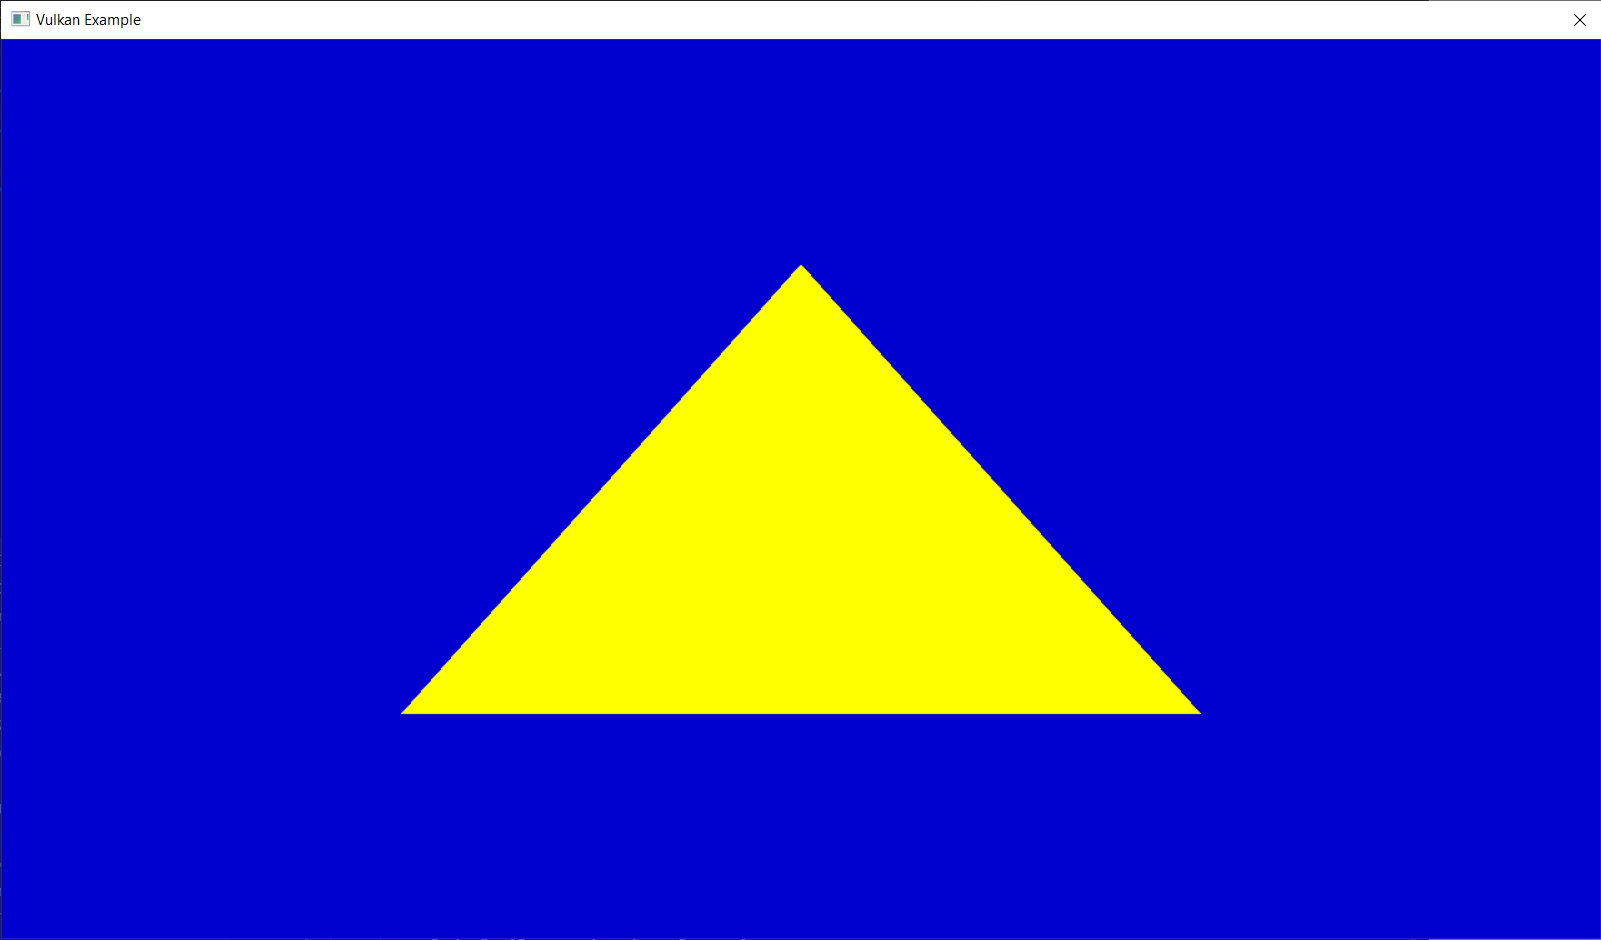
\includegraphics[scale=0.20]{images/ChTriangle/Triangle.png}
    \caption{Rendering our triangle}
    \label{fig::ClearWindow}
\end{figure}

\subsection{Record New Commands Into Our Command Buffer}

Now that we have created our pipeline state object we can use it
to set the graphics pipeline current state.
Then we can tell our graphics pipeline to draw three vertices.
This will lead to our triangle being rendered.

\begin{minipage}{\linewidth}{\noindent}
    \lstinputlisting[
        language=C++,
        caption={Rendering our triangle},
        label={lst::RenderTriangle}
        ]{src/ChTriangle/RenderTriangle.cpp}
\end{minipage}

\chapter{Shader Local Data: Vertices}

TODO: intro ...

\section{Vertex Data}

In this section we define the vertex data we need to draw our triangle.
We first define the structure of a single vertex.
After that we lay out the vertices of our triangle.

\subsection{Vertex}

Here we define the structure of our vertices.
In this case, our vertex will store its 2D position in normalized device coordinates.
It will also store its color.

\begin{minipage}{\linewidth}{\noindent}
    \lstinputlisting[
        language=C++,
        caption={What data we store per vertex},
        label={lst::PositionColorVertex}
        ]{src/ChVertices/PositionColorVertex.cpp}
\end{minipage}

\subsection{Vertex Data}

Since we want to draw a triangle, we specify three vertices.
These vertices are the ones that will be later uploaded to our GPU and be used
for rendering.

\begin{minipage}{\linewidth}{\noindent}
    \lstinputlisting[
        language=C++,
        caption={The vertices that our application will use},
        label={lst::PositionColorVertices}
        ]{src/ChVertices/PositionColorVertices.cpp}
\end{minipage}

\section{Shaders}

Since we have changed the structure of our vertices and we also
upload the vertex data to the GPU from our application,
we have to change our vertex shader.
Since our vertices also specify their color, we also change our fragment shader.

\subsection{Vertex Shader}

Our vertex shader takes as input a position value and a color value.
We also want to pass our vertex color to our fragment shader.
For this reason, our vertex shader defines an additional output variable for
the fragment color.

\begin{minipage}{\linewidth}{\noindent}
    \lstinputlisting[
        language=C++,
        caption={Our new vertex shader},
        label={lst::PositionColorShaderVertex}
        ]{src/ChVertices/PositionColorShader.vert}
\end{minipage}

\subsection{Fragment Shader}

Our fragment shader now takes as input the fragment's color.
We use this value to color our fragment.

\begin{minipage}{\linewidth}{\noindent}
    \lstinputlisting[
        language=C++,
        caption={Our new fragment shader},
        label={lst::PositionColorShaderFragment}
        ]{src/ChVertices/PositionColorShader.frag}
\end{minipage}

\section{Upload Vertex Data To The GPU}

In order to use our vertex data to render our triangle, we have to upload it
to the GPU for it to be used by our shaders.

\subsection{Understanding The Problem}

Uploading our vertex data to the GPU means that we have to copy it
from the memory that our application uses, to the memory that our GPU uses.
In practice, this means that we have to transfer data from our RAM to our GPU.
Here arises a question: to what kind of GPU memory do we upload
our vertex data?

Modern GPUs have two kinds of memory.
One kind of memory is the one that is host visible.
This means that it can be mapped to the application's address space.
Hence it's visible from our application.
The other kind of memory is the one that is device local.
This means that it cannot be mapped to our application's address space.

Host visible memory is slower.
This is due to the fact that it must be visible from both CPU side and GPU side.
This requires particular care from the GPU driver to keep the data consistent.

Device local memory is orders of magnitude faster.
This is due to the fact that in can only be accessed from the GPU.

Keeping in mind that our vertex data doesn't change at run time and that
we use our vertex data every frame, we really would love to use the fastest memory
possible.
The problem is that we still need to upload said data to the GPU, and to accomplish
this task we need to use host visible data.

\subsection{Our Solution: Idea}

One solution to this problem is to use two buffers.
One buffer, called a staging buffer, will use host visible memory.
We use this staging buffer to upload data to the GPU.

We then use another buffer that will use device local memory.
After uploading our data to the staging buffer, we issue a memory transfer command
to our GPU.
In this command we say that we want to copy our data from the former buffer to
the latter.
This latter buffer will be the one that our GPU use as a vertex buffer.

\subsection{Hot To Create A Buffer}

Before seeing the implementation of our solution we need to know how to cerate
a buffer using Vulkan.
We first create a buffer object.
Then, we allocate our buffer memory.
Finally, we bind our buffer memory to our buffer object.

\subsubsection{Create Buffer Object}

Here, the only interesting parameter is \texttt{sharingMode}.
It is a value specifying the sharing mode of the buffer when it will
be accessed by multiple queue families.
Since all our buffers will only be used by our graphics queue, we use the more
performant exclusive sharing mode.

\begin{minipage}{\linewidth}{\noindent}
    \lstinputlisting[
        language=C++,
        caption={Create a buffer object},
        label={lst::CreateBuffer}
        ]{src/ChVertices/CreateBuffer.cpp}
\end{minipage}

\subsubsection{Allocate Buffer Memory}

Our buffer memory allocation goes as follows.
We first query the memory requirements for our buffer.
Then, we fill a \texttt{VkMemoryAllocateInfo} struct.
This struct lets us configure our buffer memory allocation.
Finally, we call \texttt{vkAllocateMemory}.

\begin{minipage}{\linewidth}{\noindent}
    \lstinputlisting[
        language=C++,
        caption={Allocate buffer memory},
        label={lst::AllocateBufferMemoy}
        ]{src/ChVertices/AllocateBufferMemoy.cpp}
\end{minipage}

While we are filling in our \texttt{VkMemoryAllocateInfo} struct, we need to fill
the \texttt{memoryTypeIndex} field.
It is an index identifying a memory type from the \texttt{memoryTypes}
array of the \texttt{VkPhysicalDeviceMemoryProperties} structure.
To determine the correct value for this field we use an auxiliary function
called \texttt{FindMemoryType}.


This function tries to find an appropriate memory type index that
refers to a memory type
that is supported by our physical device and that satisfies our memory property
requirements.

\subsubsection{Bind Buffer Object And Memory}

We use \texttt{vkBindBufferMemory} to bind the buffer's object and memory together.

\subsection{Our Solution: Implementation}

\subsubsection{Create A Staging Buffer}

\subsubsection{Upload Vertex Data To The Staging Buffer}

\subsubsection{Create The Vertex Buffer}

\subsubsection{Allocate Command Buffer}

\subsubsection{Record Compy Command}

\subsubsection{Submit Command Buffer}

\subsubsection{Wait For The Command Buffer Execution To Finish}

\subsubsection{Cleanup}

\subsection{Review The Process}

\section{Pipeline Vertex Input State}

\section{Draw Using Our Vertex Data}

\chapter{Shader Global Data: Uniforms}

TODO: intro ...

\section{Uniform Data}

In this section we define the uniform data that we will use to
draw our triangle.

\subsection{Uniforms}

To draw our triangle we need three uniforms:
a model matrix,
a view matrix,
and a projection matrix.

\begin{minipage}{\linewidth}{\noindent}
    \lstinputlisting[
        language=C++,
        caption={Data that will be globally available to our shaders},
        label={lst::Uniforms}
        ]{src/ChUniforms/Uniforms.cpp}
\end{minipage}

\subsection{Uniform Buffer Data}

In order to draw our triangle, we have to specify the model, the view and the
projection matrices.
Unlike vertex data, which remains unchanged throughout the execution of
our application, uniform data usually changes frame by frame.
Hence, we need to upload such data during or main loop.

We use our model matrix to continuously rotate the triangle based on the
amount of time since the application has started.

We use our view matrix to represent a camera with position at coordinates
$(2, 2, 2)$, looking at $(0, 0, 0)$ and with $(0, 0, 1)$ as up vector.

We use our projection matrix to define the frustum of our camera.
Here we use a perspective projection with a field of view of $45$ degrees,
an aspect ratio based on the swapchain image, a near and far planes of
$0.1$ and $10$ respectively.

\begin{minipage}{\linewidth}{\noindent}
    \lstinputlisting[
        language=C++,
        caption={Updating uniforms during the application's main loop},
        label={lst::UpdateUniforms}
        ]{src/ChUniforms/UpdateUniforms.cpp}
\end{minipage}

\subsection{Vertex Shader}

We must update the vertex shader for us to use our uniform data.
In our case, we use a single uniform buffer containing our uniforms.
We multiply the vertex position with our matrices.
This transforms the vertex position.
This transformation is defined by our matrices.

This is the usual way in which we change our vertex data.
Instead of directly modifying our vertex data, we use one or more matrices
that define the transformation we want.
This computation is very fast because it's executed concurrently on our GPU.

\begin{minipage}{\linewidth}{\noindent}
    \lstinputlisting[
        language=C++,
        caption={Vertex shader that uses our uniforms},
        label={lst::UniformsVertexShader}
        ]{src/ChUniforms/UniformsVertexShader.vert}
\end{minipage}

\section{Upload Uniform Data To The GPU}

We use a buffer to upload the uniform data to the GPU.
Such buffer is called a uniform buffer.

\subsection{Define The Uniform Buffer}

Before creating our uniform buffer, we declare its layout.
In our case, since we have three uniforms, we pack them
together inside our uniform buffer.

\begin{minipage}{\linewidth}{\noindent}
    \lstinputlisting[
        language=C++,
        caption={Uniform buffer definition},
        label={lst::UBO}
        ]{src/ChUniforms/UBO.cpp}
\end{minipage}

\subsection{Create The Uniform Buffer}

\subsection{Upload Uniform Data}

\subsection{Uniform Buffer Data Alignment}

\section{Descriptor Set Layout}

\subsection{Update Our Pipeline Layout}

\section{Descriptor Set}

\section{Draw Using Our Uniform Data}

\chapter{Depth Testing}

Suppose we are drawing more than one object.
To correctly draw them on the screen we have to worry about
the order in which we execute our draw operations.
In particular, to get a realistic image, we must draw
them in descending order based on their distance from the camera.
Although this solution works, it would require us to sort
every object that is going to be rendered by depth.
If there are moving objects, we may have to sort them every frame.
If there are a lot of them, the sorting may require a considerable
amount of time, decreasing the application's framerate.
This solution also causes problems when two objects overlap.
In this case, it's not possible to determine which one
to render first without having graphical artifacts.

An alternative solution that doesn't suffer from the drawbacks
illustrated earlier, is using a depth buffer.
A depth buffer is an image that stores depth data for every pixel.
Every time the rasterizer produces a fragment, the depth test will
check if the new fragment is closer than the previous one.
If it isn't, then the new fragment is discarded.
A fragment that passes the depth test writes its own depth to the
depth buffer.

\begin{figure}[ht]
    \centering
    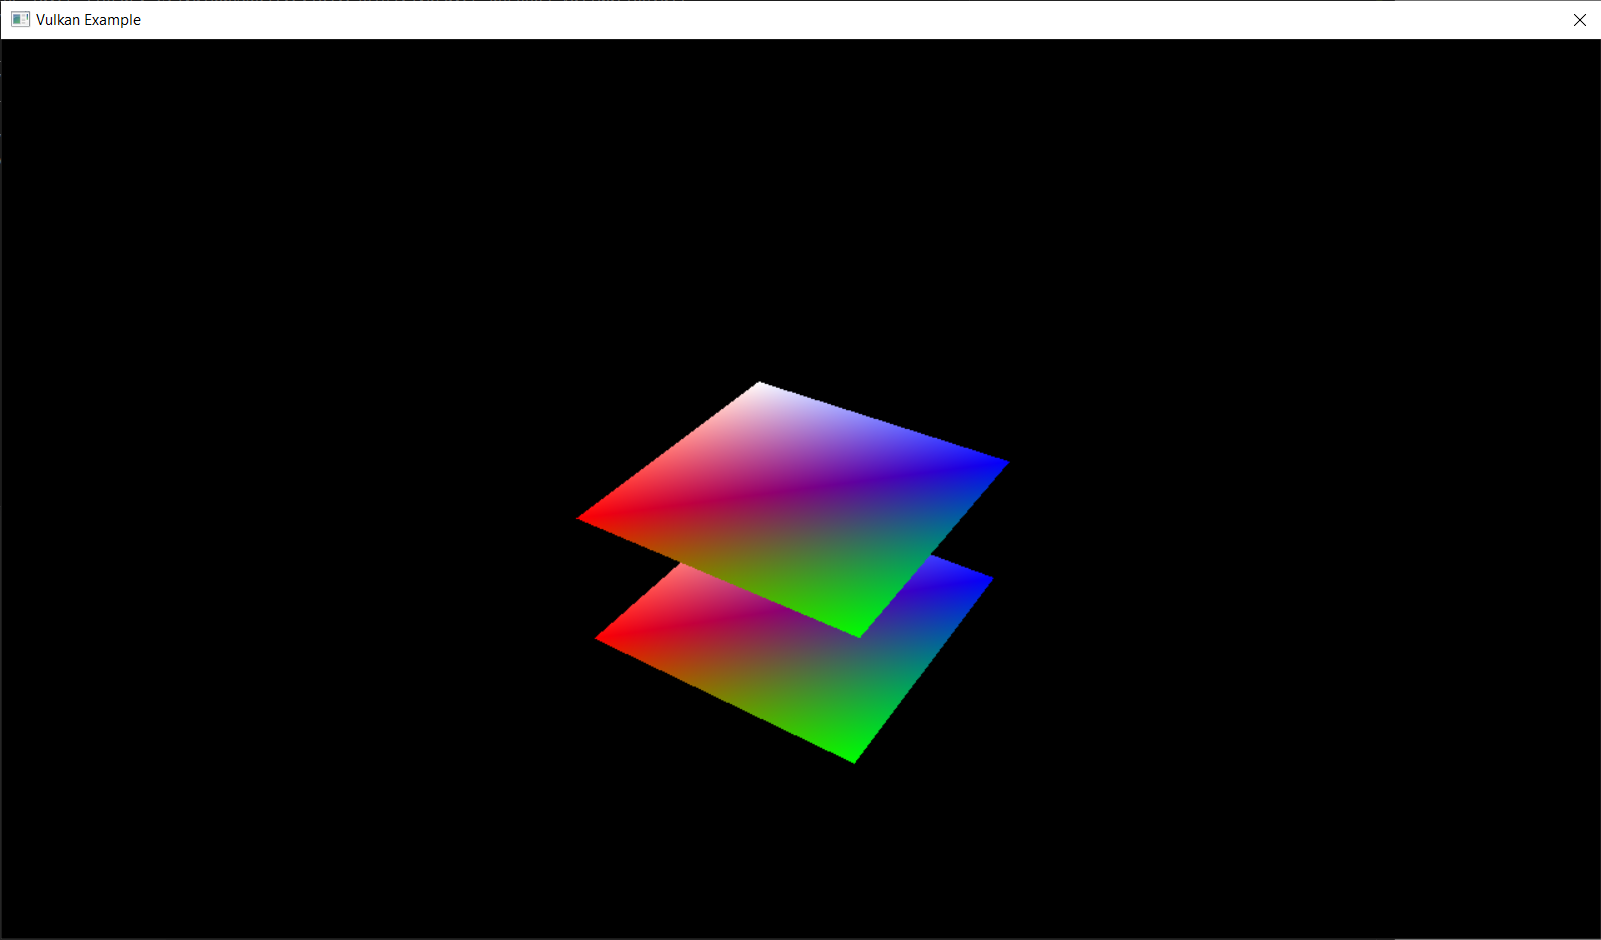
\includegraphics[scale=0.20]{images/ChDepthTesting/DepthTesting.png}
    \caption{Rendering two quads using a depth buffer}
    \label{fig::DepthTesting}
\end{figure}

\section{Creating A Depth Buffer}

Creating a depth buffer means creating an image and using
it as a depth buffer during our rendering operation.
First we must know how to create an image using Vulkan.

\subsection{Creating An Image}

Crating an image in Vulkan consists of four steps.
We first create a \texttt{VkImage} object.
Then, we allocate some memory for our \texttt{VkImage}.
We do this creating a \texttt{VkDeviceMemory} object.
Once we have both the image object and memory, we bind
them together using \texttt{vkBindImageMemory}.
Finally, in order to use the image we have created, we
create a \texttt{VkImageView} on it.

\subsubsection{VkImage}

To create a \texttt{VkImage} we use \texttt{vkCreateImage}.
Here we are creating a 2D image of a given \texttt{width}
and \texttt{height}.
We also specify the image \texttt{format} and \texttt{tiling}.
These two values define the data that the image stores per pixel
and how it's layed out in memory.
Finally, we also specify the image's \texttt{usage}.
The images that we create manually will always be used only
by our graphics queue.
Thus, we use the more performant exclusive sharing mode.

\begin{minipage}{\linewidth}{\noindent}
    \lstinputlisting[
        language=C++,
        caption={Create image object},
        label={lst::CreateImage}
        ]{src/ChDepthTesting/CreateImage.cpp}
\end{minipage}

\texttt{imageType} tells Vulkan with what kind of coordinate
system the pixels in the image are going to be addressed.
\texttt{tiling} can have one of two values: linear or optimal.
With linear tiling, pixels are laid out in row-major order.
With optimal tiling, pixels are laid out in an implementation
defined order for optimal access.
\texttt{usage} has the same semantics as the one during buffer creation.

\subsubsection{VkDeviceMemory}

We allocate some memory for a image object using \texttt{vkAllocateMemory}.
Allocating image memory is the same as allocating buffer memory.

\begin{minipage}{\linewidth}{\noindent}
    \lstinputlisting[
        language=C++,
        caption={Allocate image memory},
        label={lst::AllocateImageMemory}
        ]{src/ChDepthTesting/AllocateImageMemory.cpp}
\end{minipage}

\subsubsection{VkImageView}

We create an image view using \texttt{vkCreateImageView}.
Here, we create a 2D view on an image object, specifying
how to interpret its pixel data and which image aspects
are included in the view.

\begin{minipage}{\linewidth}{\noindent}
    \lstinputlisting[
        language=C++,
        caption={Create image View},
        label={lst::CreateImageView}
        ]{src/ChDepthTesting/CreateImageView.cpp}
\end{minipage}

\texttt{format} is the format and type used to interpret pixels in the image.
\texttt{aspectMask} is a bitmask of \texttt{VkImageAspectFlagBits}
specifying which aspect(s) of the image are included in the view.

\subsection{Cleanup}

We destroy a image view with \texttt{vkDestroyImageView}.
Then we call \texttt{vkDestroyImage} and \texttt{vkFreeMemory}
to clean up the resources we acquired to create an image.

\subsection{Depth Image Creation}

Now that we know how to create an image, we can  create our depth image.
A depth image should have the same resolution as our swapchain images.
It must have an appropriate image usage to be used as a depth buffer.
It should use optimal tiling and have device local memory, supporting fast
read and write operations.
The image should have one of the following formats:
\begin{itemize}
\item \texttt{VK\_FORMAT\_D32\_SFLOAT} using $32$ bits for depth data
\item \texttt{VK\_FORMAT\_D32\_SFLOAT\_S8\_UINT} using $32$ bits for
depth data and $8$ for stencil data
\item \texttt{VK\_FORMAT\_D24\_UNORM\_S8\_UINT} using $24$ bits for
depth data and $8$ for stencil data
\end{itemize}
The most commonly used depth format is \texttt{VK\_FORMAT\_D32\_SFLOAT}.

\begin{minipage}{\linewidth}{\noindent}
    \lstinputlisting[
        language=C++,
        caption={Create Depth Image},
        label={lst::CreateDepthImage}
        ]{src/ChDepthTesting/CreateDepthImage.cpp}
\end{minipage}

\section{Depth Image Render Pass Attachment}

To use our depth buffer we must add it to our render pass as an attachment.

\subsection{VkAttachmentDescription}

Here we describe our depth buffer attachment.
The format should be the same as the depth image itself.
We want to clear it before using it for the first time.
We don't care about storing the depth data, because it will not be
used after drawing has finished.
This may allow the driver to perform additional optimizations.
When our render pass instance begins, we don't care about its previous contents.
Right before finishing our render pass instance, we want its layout to be
optimal for depth stencil operations.

\begin{minipage}{\linewidth}{\noindent}
    \lstinputlisting[
        language=C++,
        caption={Depth buffer render pass attachment description},
        label={lst::DepthBufferRenderPassAttachmentDescription}
        ]{src/ChDepthTesting/DepthBufferRenderPassAttachmentDescription.cpp}
\end{minipage}

\subsection{Attachment descriptions}

Now that we have a new attachment description, we must remember to add it to
oru attachments array.

\begin{minipage}{\linewidth}{\noindent}
    \lstinputlisting[
        language=C++,
        caption={New render pass attachments array},
        label={lst::DepthTestRenderPassAttachments}
        ]{src/ChDepthTesting/DepthTestRenderPassAttachments.cpp}
\end{minipage}

\subsection{Render Pass Subpasses}

Inside our render pass we still have a single subpass.
But, unlike before, not only we have a color attachment, but
we also have a depth stencil attachment.

Here we are saing that our depth image will be used as the subpass depth
stencil attachment.
We are also telling Vulkan to transition our depth buffer image layout to
\texttt{VK\_IMAGE\_LAYOUT\_DEPTH\_STENCIL\_ATTACHMENT\_OPTIMAL} during
this subpass.
We do this because we execute depth operations on our depth image.

\begin{minipage}{\linewidth}{\noindent}
    \lstinputlisting[
        language=C++,
        caption={New render pass subpass},
        label={lst::DepthTestRenderPassSubpass}
        ]{src/ChDepthTesting/DepthTestRenderPassSubpass.cpp}
\end{minipage}

\section{Pipeline Depth Stencil State}

We need to enable depth testing in our pipeline state object.
This is configured through a \texttt{VkPipelineDepthStencilStateCreateInfo}
struct.

Here, we are enabling depth testing.
We are also telling Vulkan to write into the depth buffer the values that
pass the depth test.
We also specify the comparison operation that decides which fragments to
keep and which to discard.
We are sticking to the convention of lower depth means closer to the camera,
so the depth of new fragments should be less.

\begin{minipage}{\linewidth}{\noindent}
    \lstinputlisting[
        language=C++,
        caption={Configure pipeline state depth testing},
        label={lst::EnableVkPipelineDepthStencilStateCreateInfo}
        ]{src/ChDepthTesting/VkPipelineDepthStencilStateCreateInfo.cpp}
\end{minipage}

\section{Depth Image Framebuffer Attachment}

We must remember to add our depth image to the framebuffer we use during
rendering.

\begin{minipage}{\linewidth}{\noindent}
    \lstinputlisting[
        language=C++,
        caption={Modify framebuffer creation},
        label={lst::DepthBufferCreateFramebuffer}
        ]{src/ChDepthTesting/DepthBufferCreateFramebuffer.cpp}
\end{minipage}

\section{Render Pass Clear Values}

Because we now have multiple attachments with
\texttt{VK\_ATTACHMENT\_LOAD\_OP\_CLEAR}, we also need to specify multiple
clear values when we begin our render pass instance.
We clear our color attachment with an opaque black color.
We clear our depth attachment with a depth value of $1.0$.

Depth values range between $0.0$ and $1.0$.
A depth value of $1.0$ means that the fragment is the furthest away from
the camera.
A depth value of $0.0$ means that the fragment is the nearest to
the camera.

\begin{minipage}{\linewidth}{\noindent}
    \lstinputlisting[
        language=C++,
        caption={Render pass clear values},
        label={lst::AttachmentsClearValues}
        ]{src/ChDepthTesting/AttachmentsClearValues.cpp}
\end{minipage}

\chapter{Setting Up A Scene}

In this chapter we see how to lay out different objects into a virtual
world, i.e. a scene.
To do this, we introduce the concept of entity.
At the end of the chapter, we see how to set up a simple scene.

\begin{figure}[ht]
    \centering
    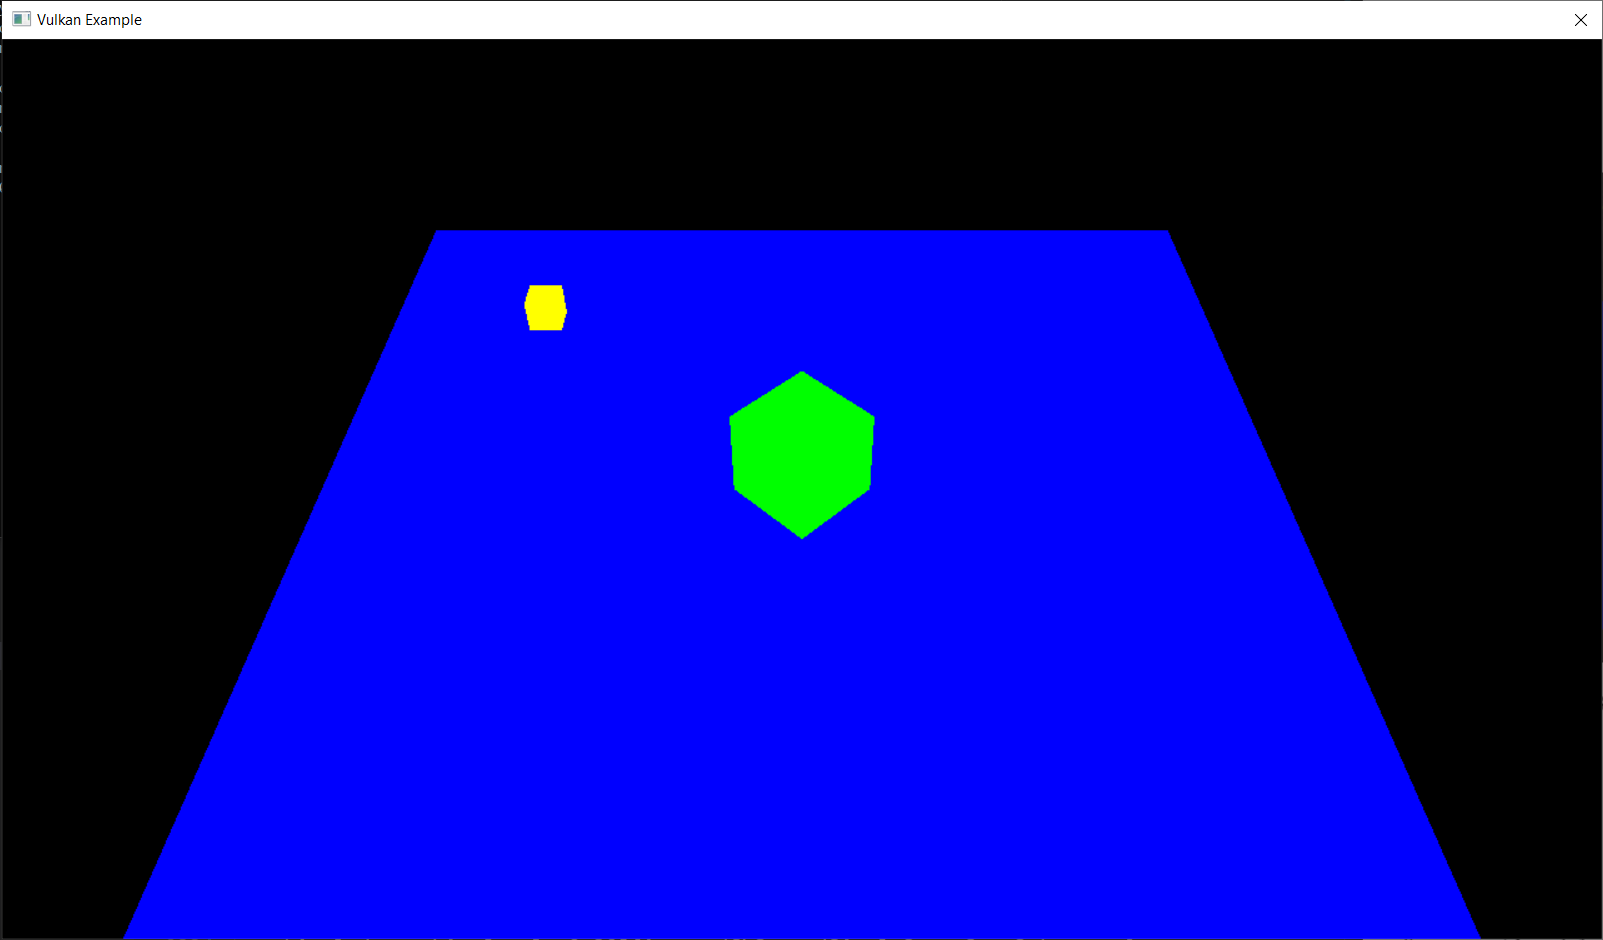
\includegraphics[scale=0.20]{images/ChScene/SimpleScene.png}
    \caption{Define and render a simple scene}
    \label{fig::SimpleScene}
\end{figure}

\section{Why Do We Need Entities?}

Suppose we want to render two squares like we did here \ref{fig::DepthTesting}.
We could, for example, use the following vertex data.

\begin{minipage}{\linewidth}{\noindent}
    \lstinputlisting[
        language=C++,
        caption={Vertices for drawing two squares},
        label={lst::TwoQuadsVertexData}
        ]{src/ChScene/TwoQuadsVertexData.cpp}
\end{minipage}

This is what we have done in all previous chapters.
We have rendered our objects directly using their vertex positions.
Although this works, it's obviously not a flexible solution.

Those of you with a keen eye have surely noticed
that our squares almost have the same vertices.
The only difference being in the $z$ coordinates.
Drawing two squares means drawing two instances of the same geometric data.
Why would we need to repeat the same data twice, just with some slight variations?
There is no reason to do it.
We can use matrices to define the transformations we want to apply to each object.
For one square we could use a matrix that doesn't apply any transformation.
For the other square we could use a matrix that translates the vertices downwards.

There is a catch.
Now, our objects are not only defined by their vertex data.
They also have a position, a rotation, etc.
We also observe that, if possible, our objects can share the same vertex data.
We should do this to avoid redundancy and to make our program more efficient.
We introduce the concept of entity to deal with this situation.

\section{Entity}

An entity is simply a collection of all the data that is necessary to place
an object in the scene and to draw it accordingly.

\subsection{Entity Positional Data}

We now have an idea of the nature of entities.
We can start by defining all the data necessary
to place an entity into a scene.

Let's start with an example.
We can have a cube placed at $(0, 0, 0)$, the origin of our scene.
We could place another cube at $(5, 3, 0)$ and rotate it by $30$
degrees around the $x$ axis and by $60$ degrees around the $z$ axis.
We could also place another cube around the scene and scale it by a factor
of $10$ to make it bigger.

From this example, we can see that our entities have three main properties
that define how the entity is contextualized inside a scene:
\begin{itemize}
    \item a 3d vector that represents its position inside the scene
    \item a 3d vector that represents its rotations around the $x, y$ and $z$ axis
    \item a scalar that represents its scale
\end{itemize}

\begin{figure}[ht]
    \centering
    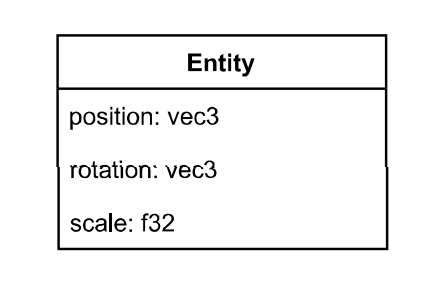
\includegraphics[scale=0.50]{images/ChScene/EntityPositionalData.png}
    \caption{Entity positional data}
    \label{fig::EntityPositionalData}
\end{figure}

\subsection{Entity Rendering Data}

In our previous example, we have talked about placing cubes around a scene.
Earlier we have discussed that entities should share their vertex data if possible.
If two or more entities are cubes, they could share the same vertex data.
In our case, sharing vertex data means using the same vertex buffer.
We know that a vertex buffer is used in tandem with a pipeline state object for
drawing operations.
Because of this, sharing a vertex buffer also means sharing a pipeline state
object.
Together with the pipeline state object we should also store the pipeline's layout.

To transform our vertices from local space to world space, we use a model matrix.
We also have to use a both a view and projection matrix to transform our vertices
from world space to clip space.
We have seen how these three matrices are passed to the vertex shader as uniforms.
Hence, our entity also needs to use a uniform buffer.
Contrary to the other rendering resources, we must create such uniform for every
entity.
This is because the entity's uniform data refers to the entity itself and is not
shared with other entities.
Together with the uniform buffer we should store a pipeline descriptor set that
contains our uniform buffer resource.

\begin{figure}[ht]
    \centering
    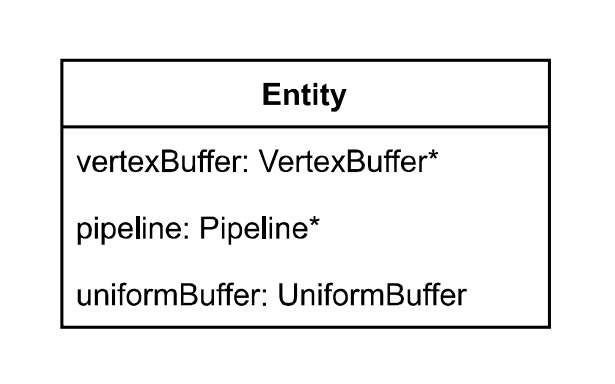
\includegraphics[scale=0.40]{images/ChScene/EntityRenderingData.png}
    \caption{Entity rendering data}
    \label{fig::EntityRenderingData}
\end{figure}

\subsection{Other Entity Data}

We have discussed all the data that it's always necessary for our entities.
Obviously, we can add more data to entities depending on our needs.
We will see multiple instances of this in the future.

\subsection{Updating Entities}

Some of our entities are not static.
This means that their properties change over time.
They could rotate, or move along one axis, for example.
The important thing to note here is that, if we want to use
our updated values in our rendering operations, we must remember
to upload the relevant data into the entity's uniform buffer.

\begin{minipage}{\linewidth}{\noindent}
    \lstinputlisting[
        language=C++,
        caption={Update entity data and uniform buffer},
        label={lst::EntityUpdate}
        ]{src/ChScene/EntityUpdate.cpp}
\end{minipage}

\subsection{Rendering Entities}

Here we can see how to use the rendering data stored in our entities
to actually draw them on the screen.

\begin{minipage}{\linewidth}{\noindent}
    \lstinputlisting[
        language=C++,
        caption={Render entity},
        label={lst::EntityRender}
        ]{src/ChScene/EntityRender.cpp}
\end{minipage}

\section{Camera}

We have seen that our entities's view and a projection matrices are computed
from \texttt{camera}.
This is a bundle of all the necessary data that is used to represent a virtual
camera inside our scene.
We need a camera in order to define the point of view from which we observe
the scene.
We could consider our camera as the eyes through which can glimpse at
our virtual world.

\subsection{Camera Data}

In our case, we use a perspective camera.
This adds perspective to the scene, making the rendered image more realistic.
In order to compute a view matrix, our camera must have:
\begin{itemize}
    \item a position, like our entities
    \item a target, i.e. a 3d vector identifying a point that the camera is looking at
    \item an up vector, i.e. a 3d vector that defines the camera's up direction
\end{itemize}
In order to compute a projection matrix, we must define our camera's frustum.
We do this using the following values:
\begin{itemize}
    \item a scalar value representing the camera's field of view
    \item a scalar value representing the camera's aspect ratio
    \item a scalar value representing a near plane
    \item a scalar value representing a far plane
\end{itemize}
All the entities that fall within the frustum will be rendered.
All the other entities will be clipped, i.e. discarded and won't be renderer.

\begin{figure}[ht]
    \centering
    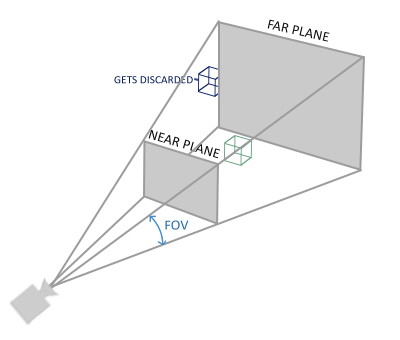
\includegraphics[scale=0.40]{images/ChScene/PerspectiveFrustum.png}
    \caption{Perspective camera frustum}
    \label{fig::PerspectiveFrustum}
\end{figure}

\begin{figure}[ht]
    \centering
    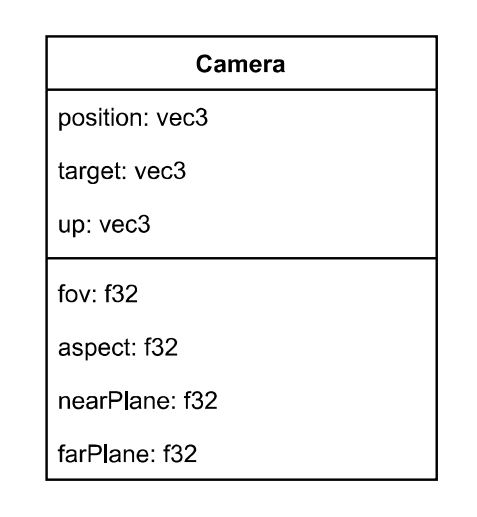
\includegraphics[scale=0.40]{images/ChScene/CameraData.png}
    \caption{Perspective camera data}
    \label{fig::CameraData}
\end{figure}

\section{Setting Up A Simple Scene}

In this section we set up a simple scene.
We do this to see the concepts we talked about in action.

\subsection{Scene Entities}

Our scene is made up by three entities.
A floor, a cube at the center of the floor, and another cube floating in the air.
The floating cube is supposed to represent a light, but here obviously we haven't
implemented lighting yet.
Don't worry about it for now, we will see how to improve our scene adding lighting
to it later.

\begin{minipage}{\linewidth}{\noindent}
    \lstinputlisting[
        language=C++,
        caption={FloorEntity},
        label={lst::FloorEntity}
        ]{src/ChScene/FloorEntity.cpp}
\end{minipage}

\begin{minipage}{\linewidth}{\noindent}
    \lstinputlisting[
        language=C++,
        caption={Cube entity},
        label={lst::CubeEntity}
        ]{src/ChScene/CubeEntity.cpp}
\end{minipage}

\begin{minipage}{\linewidth}{\noindent}
    \lstinputlisting[
        language=C++,
        caption={Light entity},
        label={lst::LightEntity}
        ]{src/ChScene/LightEntity.cpp}
\end{minipage}


TODO: show blender view of our scene

\chapter{Blinn-Phong Lighting}

In this chapter we add lighting to the scene we previously set up.
We first implement the Blinn-Phong lighting model.
After that, we refine its behavior adding materials to our objects and lights.

\section{Vulkan Related Details}

Before starting to implement the lighting model, we must clarify some technical
things related to Vulkan.

\subsection{Pipeline State Objects}

The scene's entities can be divided into two groups: the entities to which we
apply lighting, i.e. the floor and the cube; and the entities to which we
don't apply lighting, i.e. the light source itself.
This means that we must use two sets of shaders: one that implements
the Blinn-Phong lighting model, and the other that simply draws a flat color.
For this reason, we need to create two different pipeline state objects.

\subsection{Updating Our Vertex Data}

For each fragment, the lighting model needs to know the surface normal.
To solve this problem, we store, for each vertex, a normal vector.
Here we can see a visualization of the quad and cube vertex normals.

\begin{figure}[H]
    \centering
    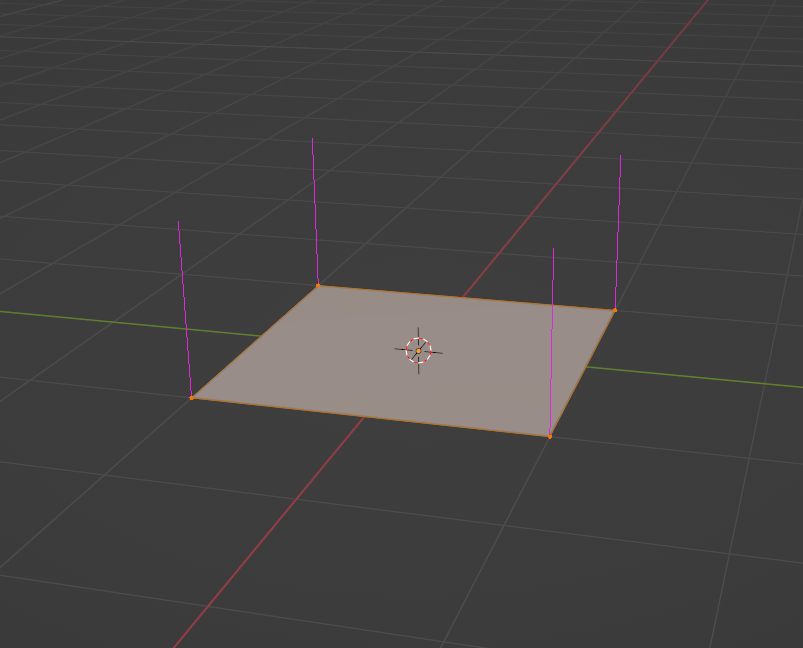
\includegraphics[scale=0.40]{images/ChBlinnPhong/QuadVertexNormals.png}
    \caption{Quad vertex normals visualization}
    \label{fig::QuadVertexNormals}
\end{figure}

\begin{figure}[H]
    \centering
    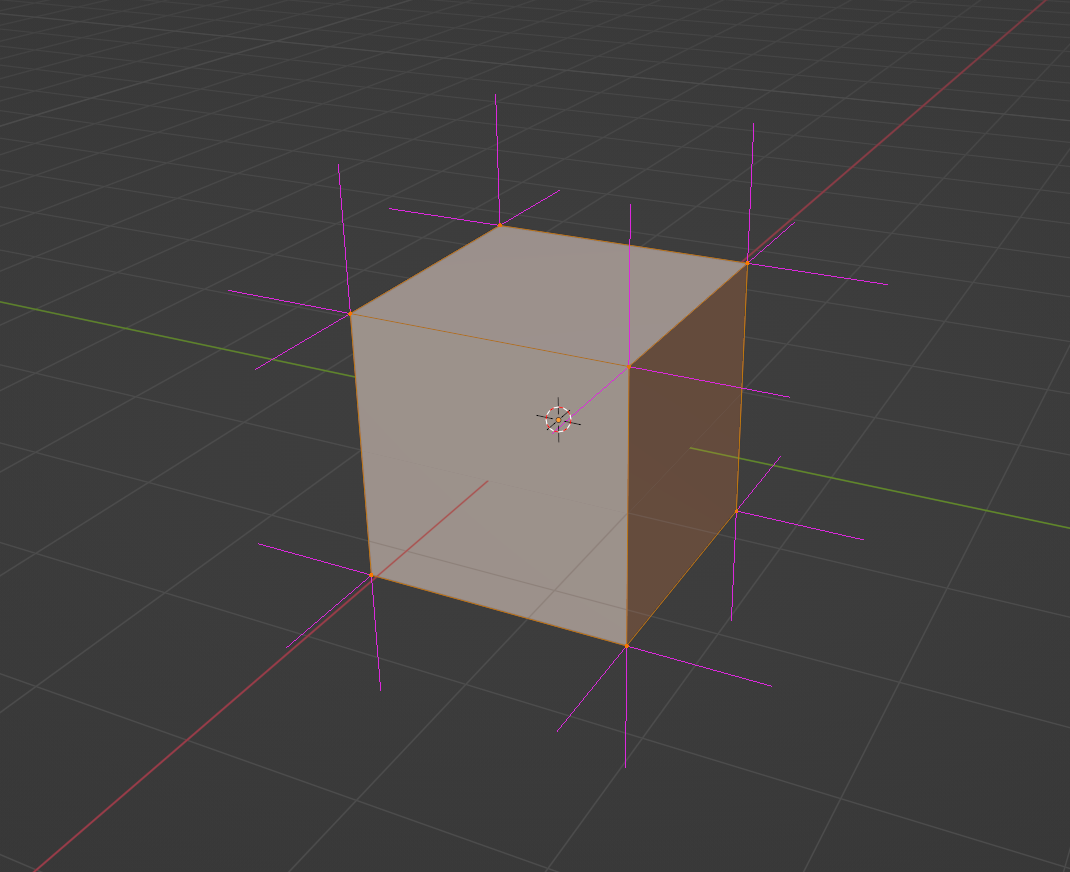
\includegraphics[scale=0.30]{images/ChBlinnPhong/CubeVertexNormals.png}
    \caption{Cube vertex normals visualization}
    \label{fig::CubeVertexNormals}
\end{figure}

\section{Blinn-Phong Lighting Model}

In computer graphics, we approximate lighting using simplified models.
The lighting model we implement here is called Blinn-Phong.
This model divides light into three components: ambient light, diffuse light and
specular light.

\subsection{Ambient Lighting}

In the real world, even when there is no apparent light source,
objects aren't completely dark.
This is because light can come from different sources around us, even if
they are not directly visible.
Indeed, light scatters and bounces in different directions.
Thus, some light sources can indirectly light our objects.
To simulate this light property, we use a small constant light value that we
add to our objects' lighting.

\begin{minipage}{\linewidth}{\noindent}
    \lstinputlisting[
        language=C++,
        caption={Computing ambient component},
        label={lst::ShadeAmbient}
        ]{src/ChBlinnPhong/ShadeAmbient.frag}
\end{minipage}

\begin{figure}[H]
    \centering
    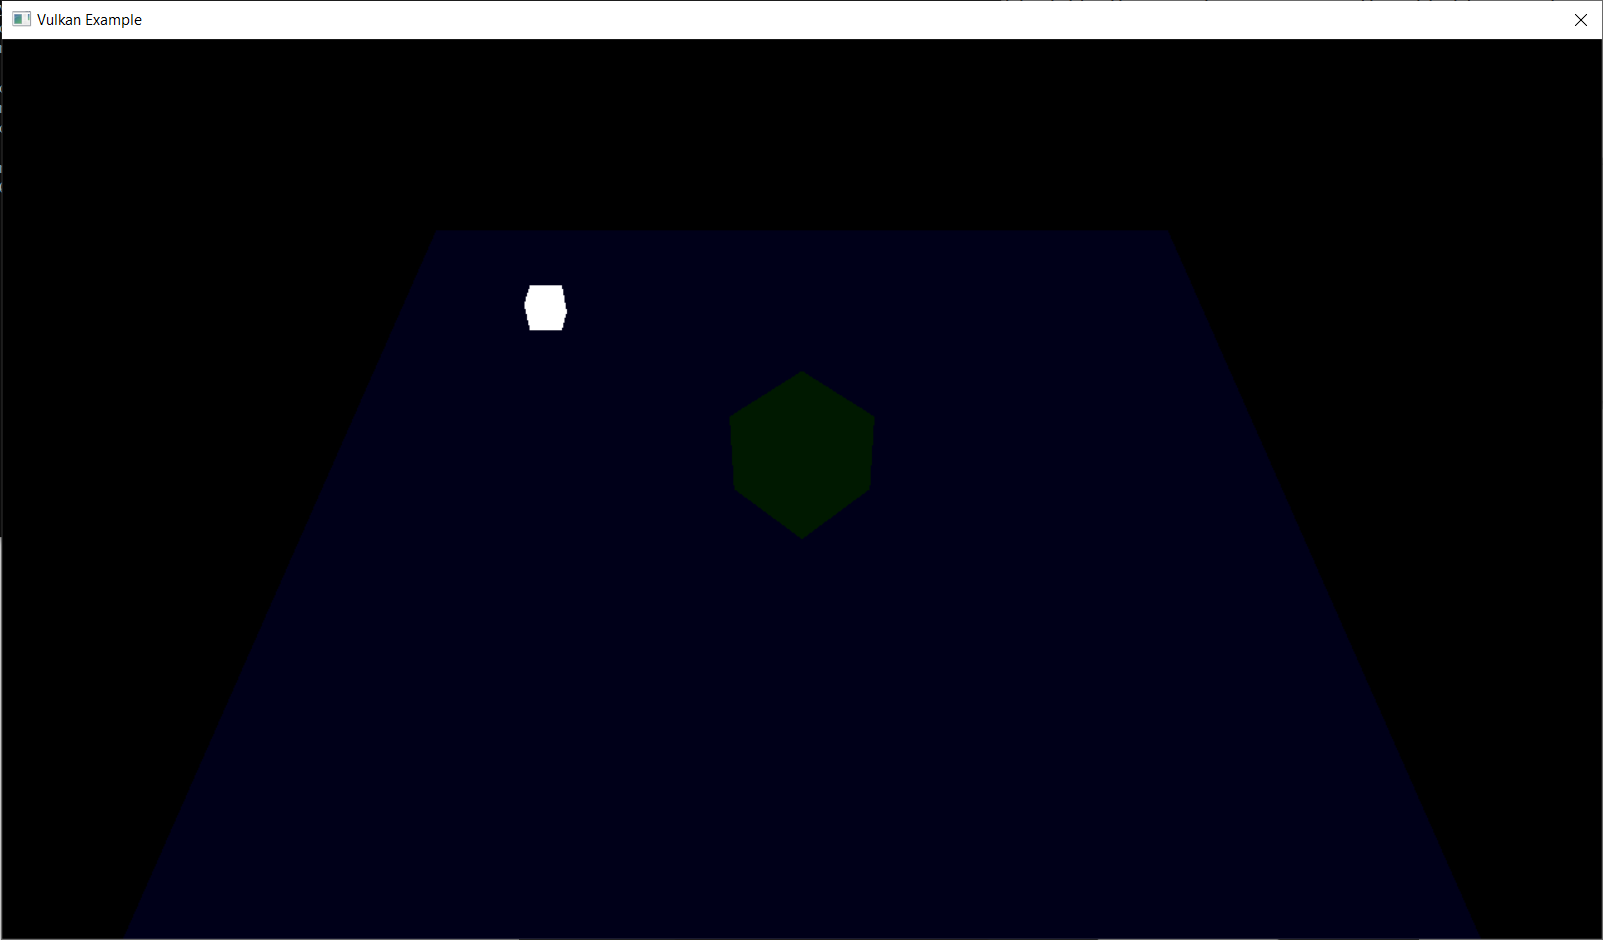
\includegraphics[scale=0.25]{images/ChBlinnPhong/SceneAmbient.png}
    \caption{Scene with ambient lighting}
    \label{fig::SceneAmbient}
\end{figure}

\subsection{Diffuse Lighting}

Diffuse lighting simulates the impact a light has on an opaque object.
In simple terms, the more a part of the object faces the light, the brighter
it becomes.
The diffuse impact is the strongest when
the angle between the surface's normal and the light ray is zero.
The diffuse impact will be zero when the angle is greater than or equal to
ninety degrees.

\begin{figure}[H]
    \centering
    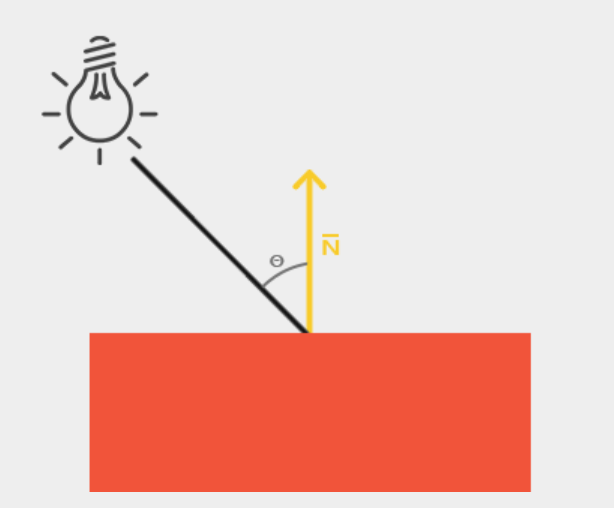
\includegraphics[scale=0.40]{images/ChBlinnPhong/DiffuseLighting.png}
    \caption{Diffuse lighting}
    \label{fig::DiffuseLighting}
\end{figure}

\begin{minipage}{\linewidth}{\noindent}
    \lstinputlisting[
        language=C++,
        caption={Computing diffuse component},
        label={lst::ShadeDiffuse}
        ]{src/ChBlinnPhong/ShadeDiffuse.frag}
\end{minipage}

\begin{figure}[H]
    \centering
    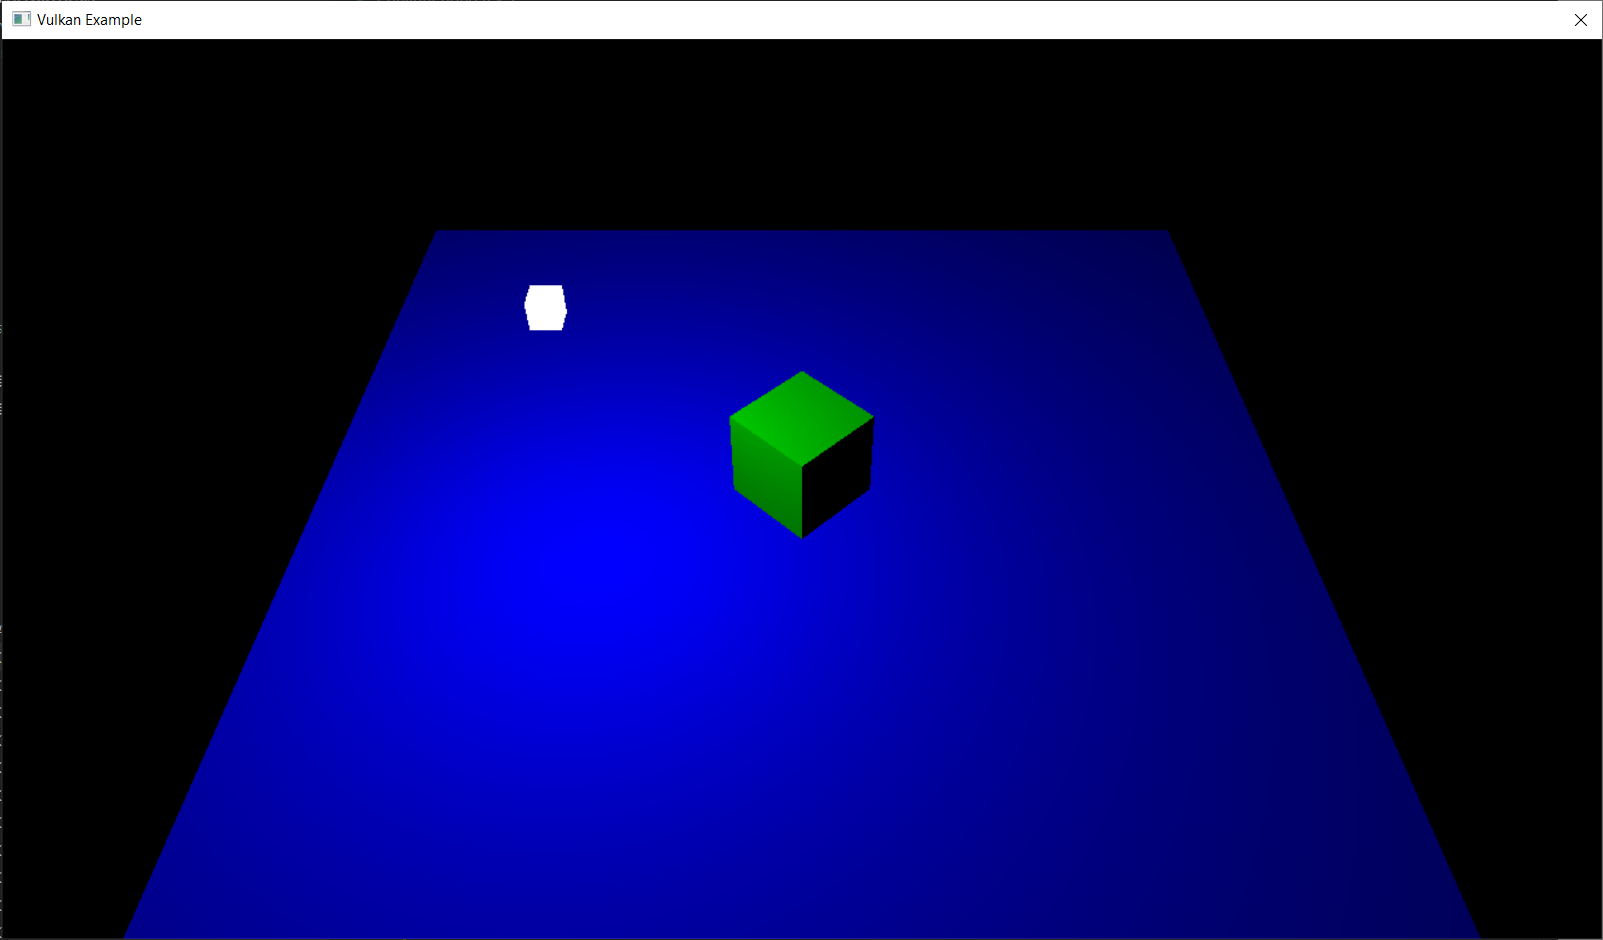
\includegraphics[scale=0.25]{images/ChBlinnPhong/SceneDiffuse.png}
    \caption{Scene with diffuse lighting}
    \label{fig::SceneDiffuse}
\end{figure}

\subsection{Specular Lighting}

Specular lighting simulates the bright spot that lights cause on shiny objects.
This spot is called specular highlight.
The specular impact is the strongest when our view direction is perfectly
aligned with the light ray that is reflected off the object's surface.
The more our view deviates form the reflected vector, the less the specular
impact will be.

To compute the specular impact we first compute a unit vector exactly
halfway between the view direction and the light direction.
The closer this halfway vector aligns with the surface's normal, the higher
the specular impact.

\begin{figure}[H]
    \centering
    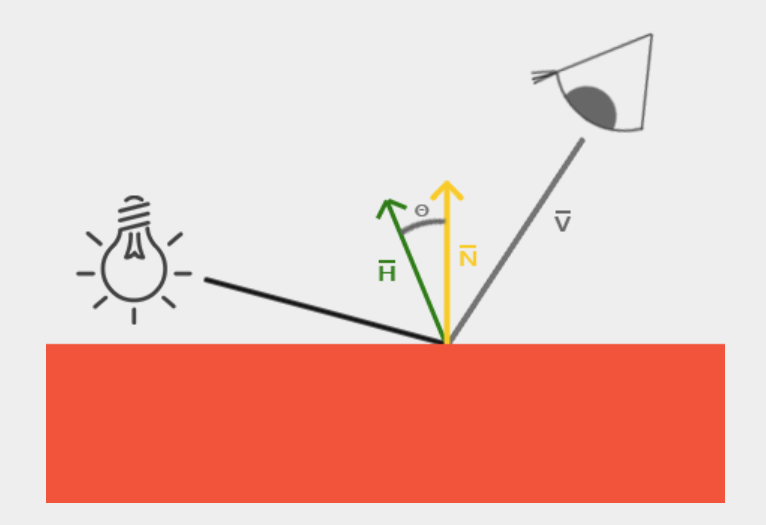
\includegraphics[scale=0.40]{images/ChBlinnPhong/SpecularLighting.png}
    \caption{Specular lighting}
    \label{fig::SpecularLighting}
\end{figure}

\begin{minipage}{\linewidth}{\noindent}
    \lstinputlisting[
        language=C++,
        caption={Computing specular component},
        label={lst::ShadeSpecular}
        ]{src/ChBlinnPhong/ShadeSpecular.frag}
\end{minipage}

\begin{figure}[H]
    \centering
    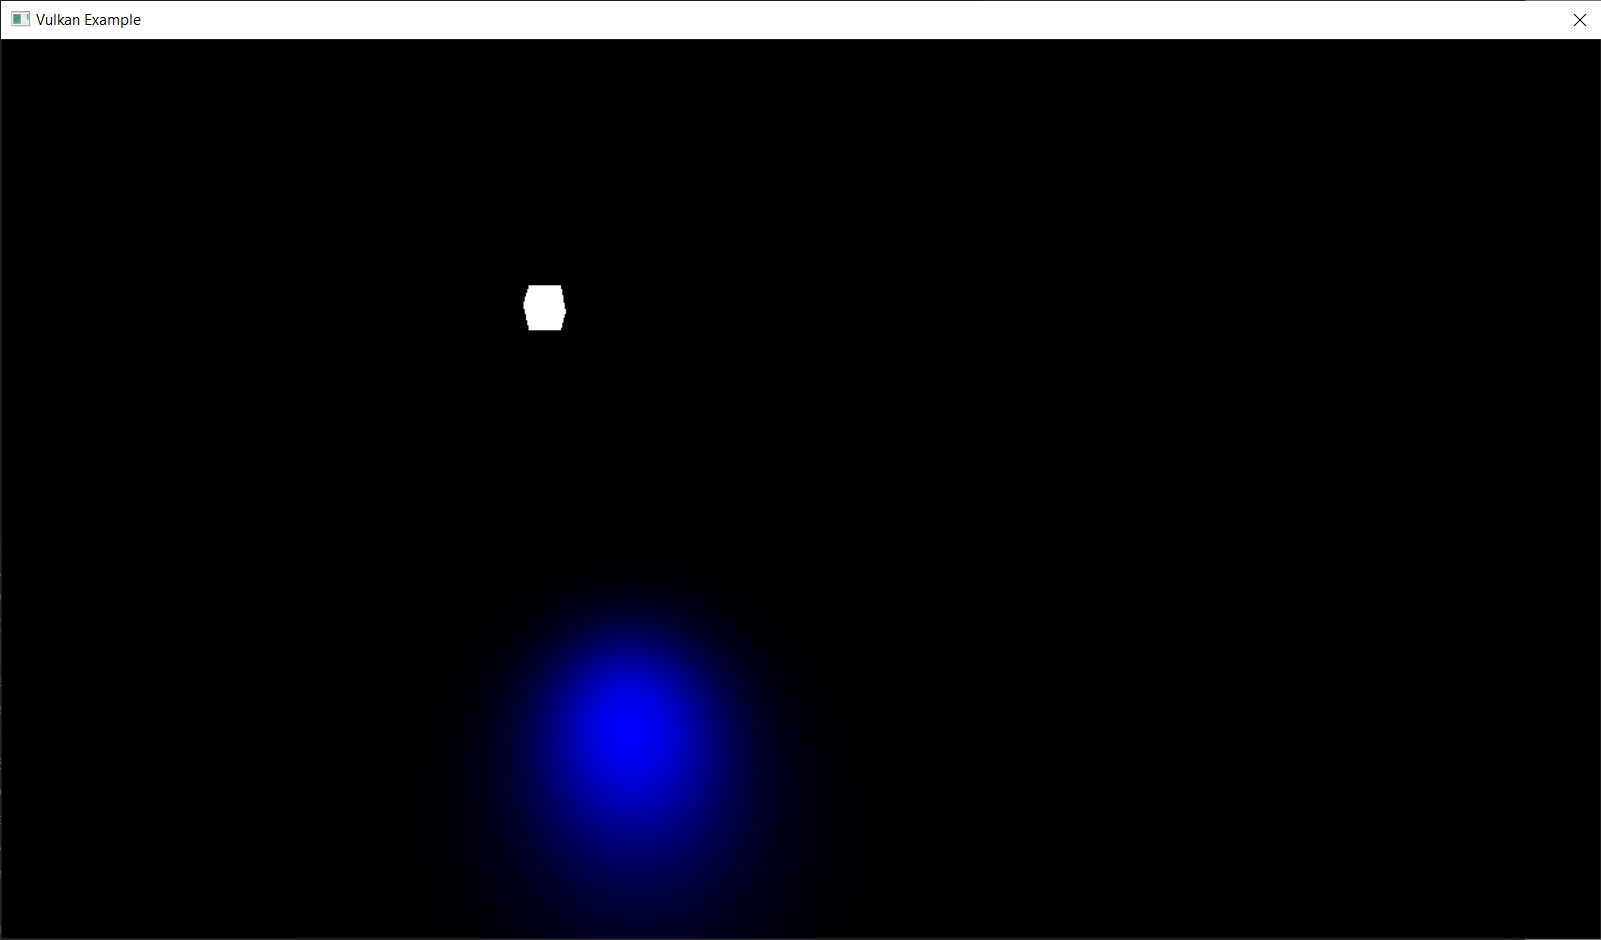
\includegraphics[scale=0.25]{images/ChBlinnPhong/SceneSpecular.png}
    \caption{Scene with specular lighting}
    \label{fig::SceneSpecular}
\end{figure}

\subsection{Putting It All Together}

Finally we can merge ambient, diffuse and specular components together.
We do this by simply adding them together.

\begin{minipage}{\linewidth}{\noindent}
    \lstinputlisting[
        language=C++,
        caption={Computing final light value},
        label={lst::ShaderMergeComponents}
        ]{src/ChBlinnPhong/ShaderMergeComponents.frag}
\end{minipage}

\begin{figure}[H]
    \centering
    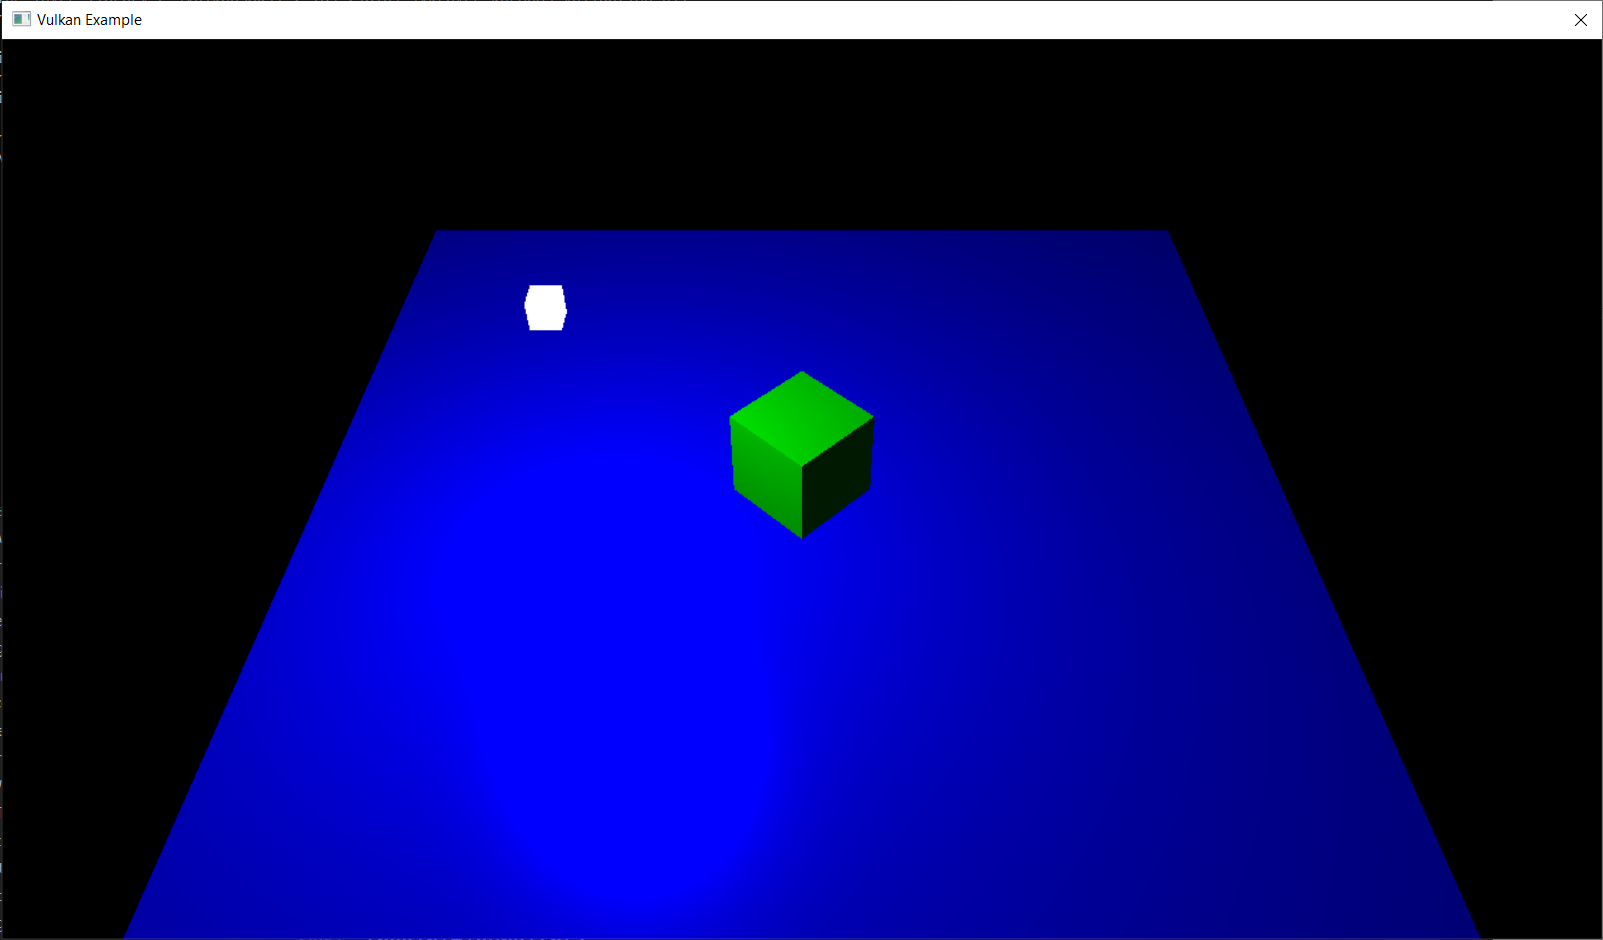
\includegraphics[scale=0.25]{images/ChBlinnPhong/SceneLit.png}
    \caption{Scene with ambient, diffuse and specular lighting}
    \label{fig::SceneLit}
\end{figure}

\section{Materials}

Real world objects have different reactions to light.
We simulate this property using materials.
We can describe a material by specifying four different properties:
one for each lighting component plus a shininess value.
We can simulate a lot of different real world materials simply using
different combinations of these four values.

\subsection{Scene Materials}

In our scene, we use two materials.
The \texttt{turquoise} material is used by the floor entity.
The \texttt{emerald} material is used by the cube entity.

\begin{minipage}{\linewidth}{\noindent}
    \lstinputlisting[
        language=C++,
        caption={Materials used in our scene},
        label={lst::Materials}
        ]{src/ChBlinnPhong/Materials.cpp}
\end{minipage}

\subsection{Blinn-Phong With Object Materials}

The ambient material property defines what color the surface reflects
under ambient lighting.
This is usually the same as the surface's color.
The diffuse material property defines the color of the surface under
diffuse lighting.
The specular material property defines the color of the specular highlight.
The shininess material property affects the specular highlight's radius.

\begin{minipage}{\linewidth}{\noindent}
    \lstinputlisting[
        language=C++,
        caption={Blinn-Phong lighting using object materials},
        label={lst::ShadeMaterials}
        ]{src/ChBlinnPhong/ShadeMaterials.frag}
\end{minipage}

\begin{figure}[H]
    \centering
    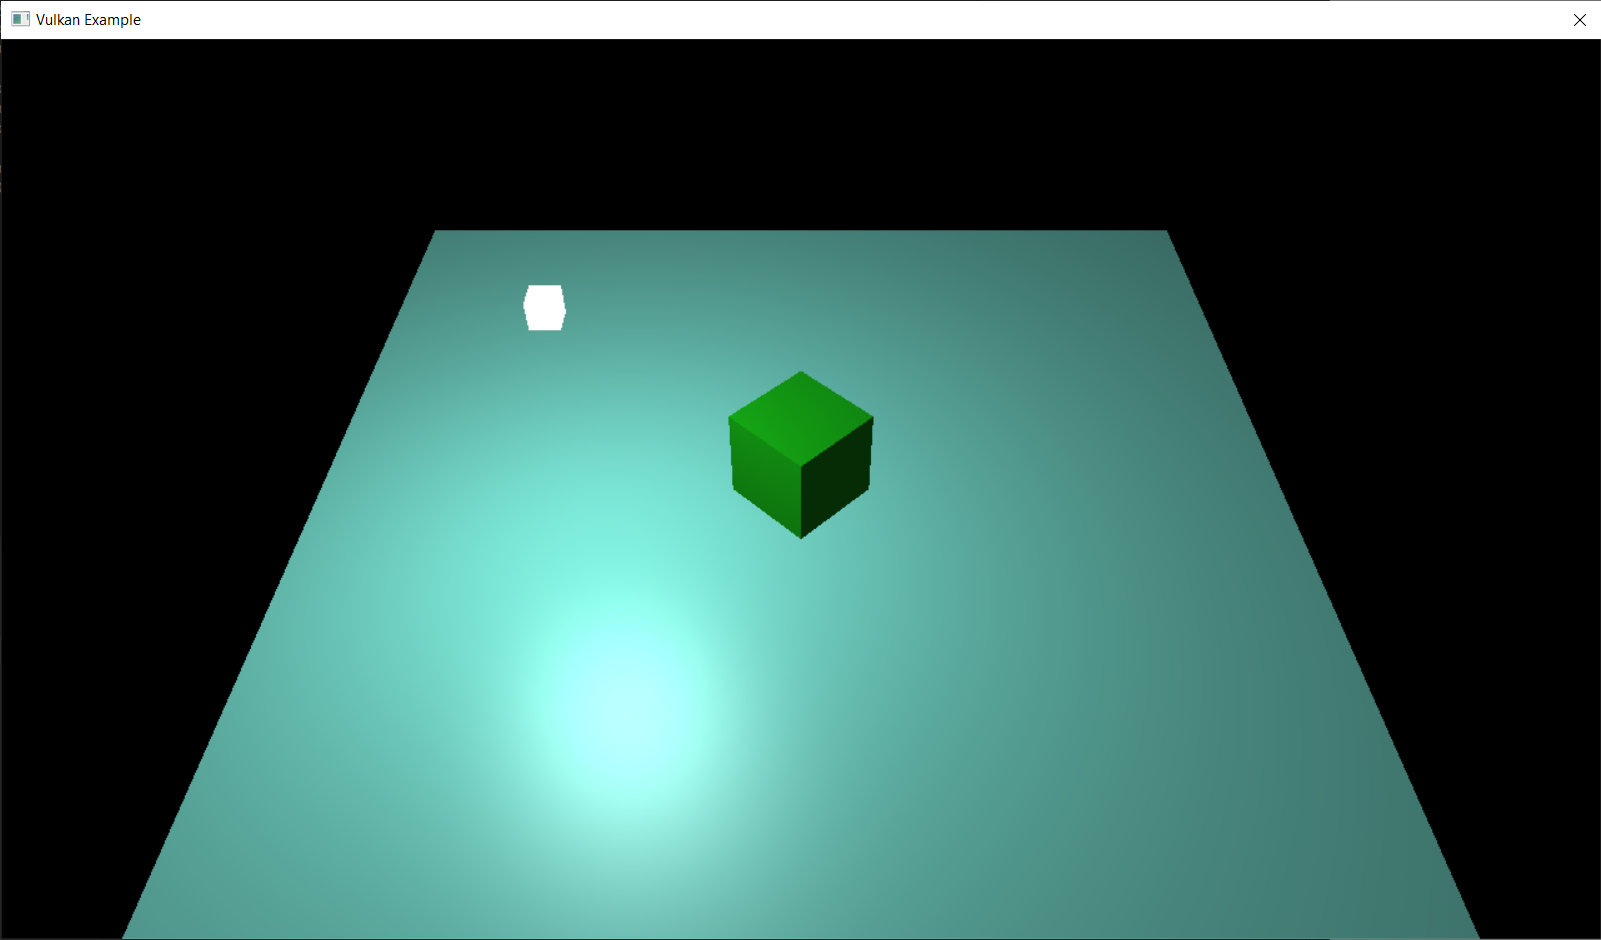
\includegraphics[scale=0.25]{images/ChBlinnPhong/SceneMaterials.png}
    \caption{Scene lighting using material properties}
    \label{fig::SceneMaterials}
\end{figure}

\subsection{Blinn-Phong With Object And Light Materials}

In the previous image, we see that the objects are too bright.
This is due to the fact that the ambient, diffuse and specular
colors are computed simply using the light's color.
Lights also have different intensities for their ambient,
diffuse and specular components.

We set the ambient component to a low intensity because we don't want the
ambient color to be too dominant.
We set the diffuse component to a slightly darkened version of the light's
color.
We set the specular component to the light's color, shining at full intensity.

\begin{minipage}{\linewidth}{\noindent}
    \lstinputlisting[
        language=C++,
        caption={Our scene light's material},
        label={lst::LightMaterial}
        ]{src/ChBlinnPhong/LightMaterial.cpp}
\end{minipage}

\begin{minipage}{\linewidth}{\noindent}
    \lstinputlisting[
        language=C++,
        caption={Blinn-Phong lighting using object and light materials},
        label={lst::ShadeLightMaterial}
        ]{src/ChBlinnPhong/ShadeLightMaterial.frag}
\end{minipage}

\begin{figure}[H]
    \centering
    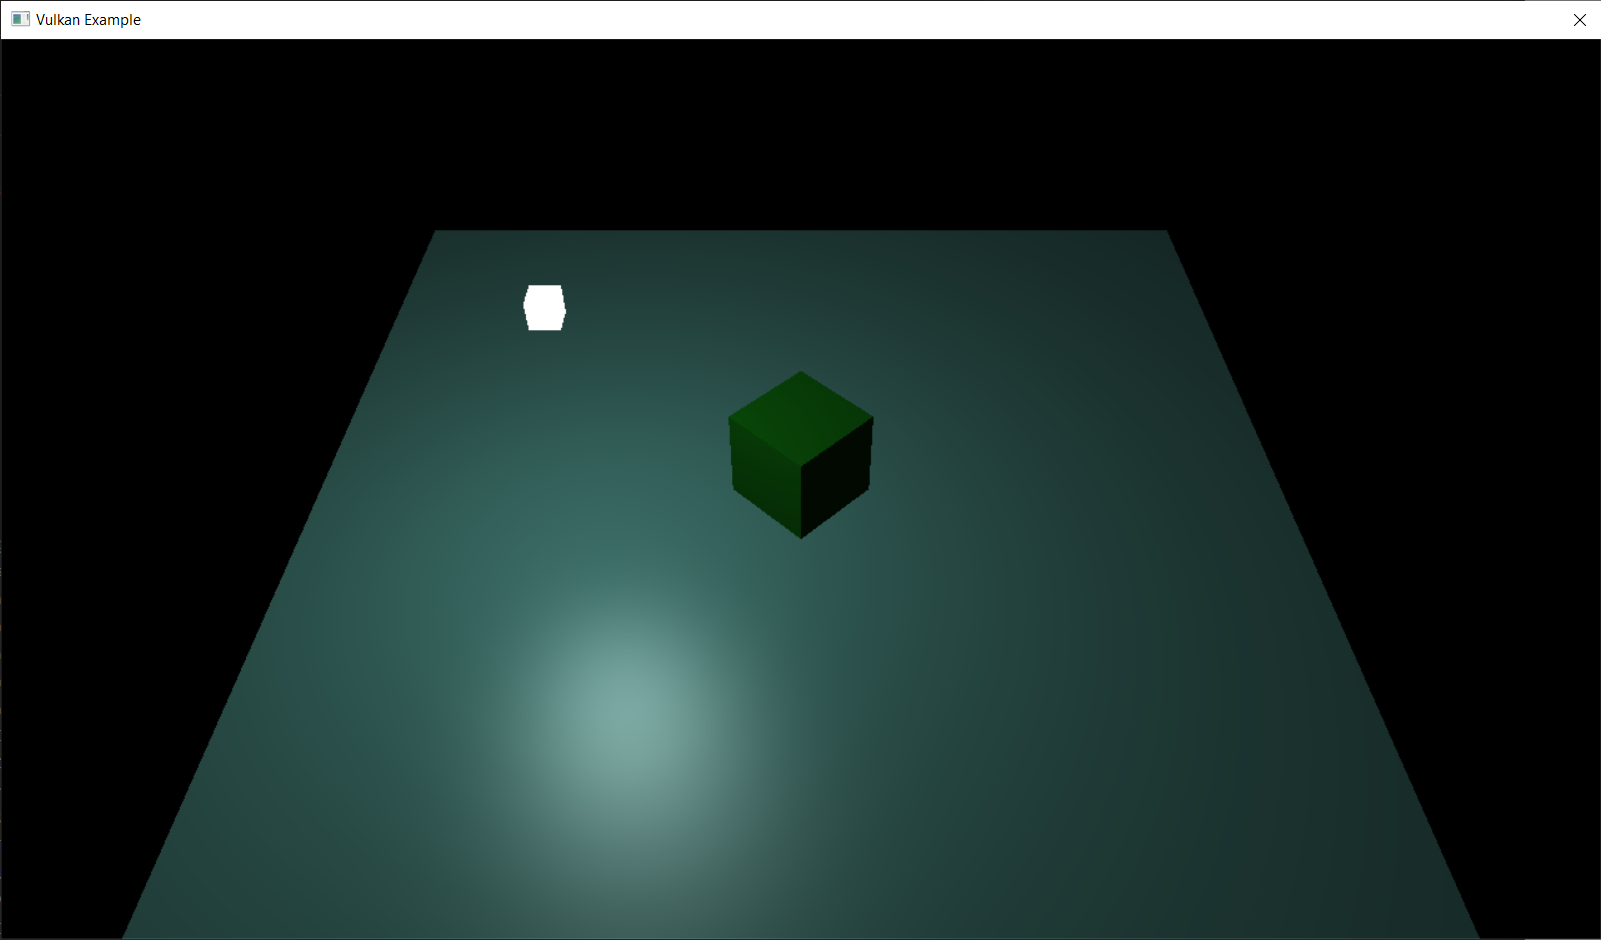
\includegraphics[scale=0.25]{images/ChBlinnPhong/SceneMaterialsLight.png}
    \caption{Scene lighting using object and light materials}
    \label{fig::SceneMaterialsLight}
\end{figure}

\chapter{Multisample Anti Aliasing}
\label{chap:MSAA}

If we examine up close the images we have rendered up to this point, we
can notice that some of our edges have a jagged saw like pattern.
This effect is called aliasing and it's the result of having to render our
images on a grid with a finite number of pixels.
We can't completely avoid this effect since screens will always have a
finite resolution.
We can, however, attenuate the issue using a technique known as multisample
anti aliasing, MSAA for short.

\begin{figure}[H]
    \centering
    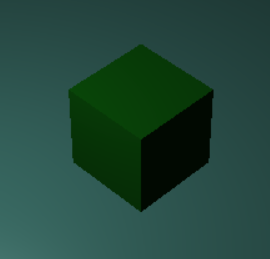
\includegraphics[scale=1.0]{images/ChMSAA/AnExampleOfAliasing.png}
    \caption{An example of aliasing}
    \label{fig::AliasingExample}
\end{figure}

\section{MSAA}

So far, we have always used only one sample per pixel.
This means that we determine its color using a single sample
point, placed at its center.
If the rendered geometry doesn't cover the sample point, the entire pixel
is left blank.
Else, if the rendered geometry covers the sample point, we color the entirety of
the pixel.
This is what causes aliasing.

\begin{figure}[H]
    \centering
    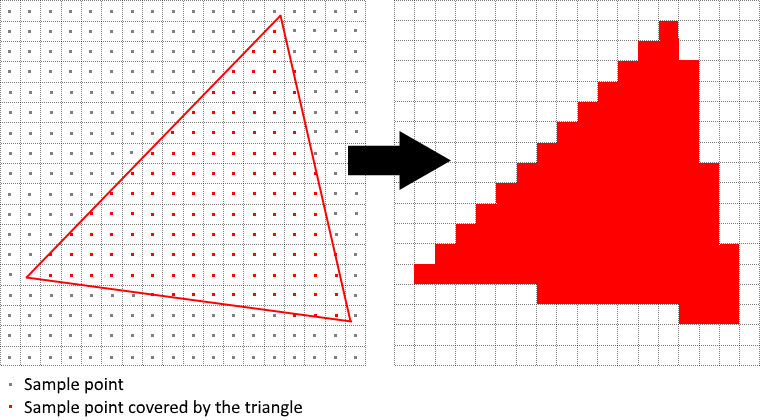
\includegraphics[scale=0.6]{images/ChMSAA/OneSamplePerPixel.png}
    \caption{Rendering using one sample per pixel}
    \label{fig::OneSamplePerPixel}
\end{figure}

\begin{figure}[H]
    \centering
    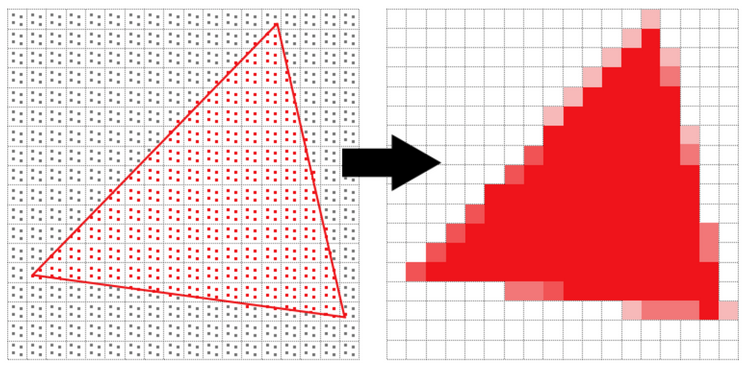
\includegraphics[scale=0.62]{images/ChMSAA/FourSamplesPerPixel.png}
    \caption{Rendering using four samples per pixel}
    \label{fig::FourSamplesPerPixel}
\end{figure}

MSAA uses multiple sample points per pixel to determine its final color.
More samples lead to better results but also mean more overhead.
For each pixel, the less the samples are covered by the geometry, the less
the geometry color contributes to the pixel final color.
Thanks to this, edges are surrounded by colors slightly lighter than the
edge's color itself.
This causes the edge to appear smooth when viewed from a distance.

\section{Adding MSAA In Vulkan}

In this section we discuss all the steps that are necessary to add MSAA
to our Vulkan application.

\subsection{Get Available Sample Count}

We must determine how many samples our hardware can use.
To do this we query the maximum number of samples for both color and depth values.
After that, we pick the highest sample count that they both support.

\begin{minipage}{\linewidth}{\noindent}
    \lstinputlisting[
        language=C++,
        caption={Determine the maximum supported sample count},
        label={lst::GetMaxMSAASampleCount}
        ]{src/ChMSAA/GetMaxMSAASampleCount.cpp}
\end{minipage}

\subsection{Create New Render Target}

Up to this point, we have always used the next swapchain image as our
render target.
The problem is that our swapchain images store only one sample per pixel.
They can't store more than one sample per pixel, because that, would make
them not presentable.
Thus, we have to create a new multisampled image that will be used
as our application's render target.

\subsubsection{Creating The Multisample Render Target}

To create our new render target, we reuse the image creation functions
we saw in earlier chapters.
The only thing different from before, is that we now pass the
number of samples that our image will store per pixel.

\begin{minipage}{\linewidth}{\noindent}
    \lstinputlisting[
        language=C++,
        caption={Create the multisample render target},
        label={lst::CreateMultisampleRenderTarget}
        ]{src/ChMSAA/CreateMultisampleRenderTarget.cpp}
\end{minipage}

\subsubsection{Update Depth Buffer Creation}

We must also remember to update the depth buffer creation.
This is because the depth buffer will also store more samples per pixel.

\subsection{Update Render Pass}

We set the color attachment and the depth attachment samples count
to \texttt{msaaSamples}.
We also change the color attachment's final layout to
\texttt{VK\_IMAGE\_LAYOUT\_COLOR\_ATTACHMENT\_OPTIMAL}.
We do this because multisampled images can't be directly presented.

\subsubsection{Add A Resolve Color Attachment}

Right now, we only have a multisampled render target and a multisampled
depth buffer.
Neither is suitable to be presented to the screen.
Because of this, we add a new color attachment to the render pass.
After finishing our rendering operations, we will resolve our render target to
this new color attachment.
This resolve color attachment is the one that will be presented to the screen.

\begin{minipage}{\linewidth}{\noindent}
    \lstinputlisting[
        language=C++,
        caption={Color resolve attachment},
        label={lst::ColorResolveAttachment}
        ]{src/ChMSAA/ColorResolveAttachment.cpp}
\end{minipage}

\subsubsection{Render Pass Attchments}

Now our render pass has three attachments.

\begin{minipage}{\linewidth}{\noindent}
    \lstinputlisting[
        language=C++,
        caption={MSAA render pass attachments},
        label={lst::MSAARenderPassAttachments}
        ]{src/ChMSAA/MSAARenderPassAttachments.cpp}
\end{minipage}

\subsubsection{Update Color Subpass Description}

We must tell to our color subpass to actually use the color resolve attachment.
To do this we update its description.

\begin{minipage}{\linewidth}{\noindent}
    \lstinputlisting[
        language=C++,
        caption={Color resolve attachment reference},
        label={lst::ColorResolveAttachmentReference}
        ]{src/ChMSAA/ColorResolveAttachmentReference.cpp}
\end{minipage}

\subsection{Update Multisampling Pipeline State}

Not only we need to create resources that are compatible with MSAA.
We also need to directly enable it while creating the pipeline state object.

\begin{minipage}{\linewidth}{\noindent}
    \lstinputlisting[
        language=C++,
        caption={Enable multisampling},
        label={lst::MSAAPipelineMultisampleState}
        ]{src/ChMSAA/MSAAPipelineMultisampleState.cpp}
\end{minipage}

\subsection{Update Framebuffer}

Now that we have updated our render pass attachments, we also must update
the attachments that are used by our framebuffers.
We use the multisample render target as the first attachment.
We use the depth buffer as the second attachment.
And we use the next swapchain image as the color resolve attachment.

\section{Side By Side Comparison}

Here we can see a side by side comparison of how MSAA influences the
rendered image's quality.
On the left we see the cube rendered without using MSAA.
On the right we see the cube rendered using MSAA.
As explained earlier, the jagged pattern gets blurred making it look
smoother.
This leads to more pleasant visuals.

\begin{figure}[H]
    \centering
    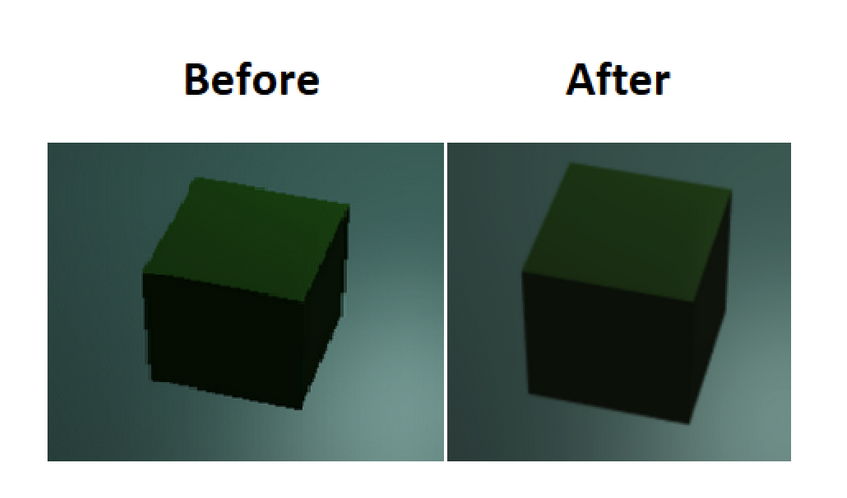
\includegraphics[scale=0.40]{images/ChMSAA/BeforeAfterMSAA.png}
    \caption{Before and after MSAA}
    \label{fig::MSAASideBySide}
\end{figure}


\chapter{Conclusion}


\appendix

\chapter{Concepts}

\section{Graphics Pipeline}
TODO: to be written ...

\section{Shaders}
TODO: to be written ...


\bibliographystyle{plain}
\nocite{*}
\bibliography{Refs.bib}

\end{document}
